\documentclass[11pt,a4paper]{article}
\usepackage{fontspec}
\IfFontExistsTF{Times New Roman}{\setmainfont{Times New Roman}}{\setmainfont{TeX Gyre Termes}}
\usepackage[a4paper,left=25mm,right=25mm,top=24mm,bottom=25mm]{geometry}
\usepackage{graphicx,booktabs,longtable,tabularx,array,multirow,caption,subcaption,float}
\usepackage{enumitem,microtype,amsmath,xcolor,fancyhdr,setspace,tikz}
\usetikzlibrary{arrows.meta,positioning,shapes.geometric}
\usepackage[unicode,colorlinks=true,linkcolor=blue!55!black,citecolor=blue!55!black,urlcolor=blue!55!black]{hyperref}
\usepackage[backend=biber,style=numeric,sorting=none]{biblatex}
\addbibresource{refs.bib}

\definecolor{navy}{HTML}{173A63}
\definecolor{blue}{HTML}{2F7ED8}
\definecolor{orange}{HTML}{E9783A}
\definecolor{soft}{HTML}{F2F6FA}
\definecolor{green}{HTML}{1F9D73}
\setstretch{1.18}
\setlength{\parindent}{0pt}
\setlength{\parskip}{5pt}
\setlist[itemize]{leftmargin=18pt,itemsep=3pt,topsep=3pt}
\setlist[enumerate]{leftmargin=20pt,itemsep=3pt,topsep=3pt}
\captionsetup{font=small,labelfont=bf}
\pagestyle{fancy}
\fancyhf{}
\fancyhead[L]{\small What Shapes Student CGPA?}
\fancyhead[R]{\small CSE 4112 Machine Learning Laboratory}
\fancyfoot[C]{\thepage}
\renewcommand{\headrulewidth}{0.4pt}
\newcolumntype{Y}{>{\raggedright\arraybackslash}X}
\newcommand{\code}[1]{\texttt{#1}}
\newcommand{\placeholder}[1]{\fcolorbox{orange}{orange!8}{\parbox{0.94\linewidth}{\textbf{TODO:} #1}}}
\newcommand{\partbanner}[1]{\clearpage\thispagestyle{empty}\vspace*{0.28\textheight}\begin{center}\color{navy}\rule{0.75\linewidth}{1.2pt}\\[12pt]{\Huge\bfseries #1}\\[12pt]\rule{0.75\linewidth}{1.2pt}\end{center}\clearpage}

\begin{document}
\begin{titlepage}
\centering
\vspace*{16mm}
{\color{navy}\rule{\textwidth}{1.5pt}}\\[12mm]
{\Huge\bfseries What Shapes Student CGPA?\\[4mm]}
{\LARGE An Engineering Student Academic Performance Dataset and Machine Learning Analysis}
\\[11mm]
{\Large CSE 4112: Machine Learning Laboratory}\\[4mm]
{\large Department of Computer Science and Engineering\\Khulna University of Engineering \& Technology}
\\[12mm]
\begin{tabular}{rl}
2107007 & Asif Jawad\\
2107008 & Rakibul Islam\\
2107012 & Md Enam E Elahi\\
2107014 & Al Mubtasim Preom\\
2107020 & Sheikh Md. Galib Mahim\\
2107030 & Md. Eftakar Jaman Arfan
\end{tabular}
\\[12mm]
\textbf{Submitted to}\\
Dr. Muhammad Aminul Haque, Professor\\
Nabil Faiyaz Sadi, Lecturer\\[8mm]
Lab Group A1\\[3mm]
14 September 2026
\vfill
{\color{navy}\rule{\textwidth}{1.5pt}}
\end{titlepage}

\pagenumbering{roman}
\section*{Abstract}
This course report documents a questionnaire dataset collected from undergraduate engineering students in Bangladesh. Two independently administered Google Forms captured the same core academic, behavioural, lifestyle, motivation, support, and study-environment concepts with small differences in wording, language, ordering, and grade-band options. The source files contain 1,126 responses: 230 from BUET, BRAC University, and CUET, and 896 from KUET. A reproducible pipeline maps both forms to a common schema, removes source-specific text differences, normalises university and department names, reconciles grade bands, records missing-value decisions, and removes 18 records without a usable CGPA target. The resulting dataset contains 1,108 cleaned student records from four universities and represents both recent SGPA and cumulative CGPA as four ordered groups from C0 to C3. The project package includes raw and cleaned tabular files, WEKA-ready ARFF files, a data dictionary, cleaning logs, descriptive figures, fixed train/test indices, model-output tables, and executable notebooks. These resources support reuse in educational data analysis, questionnaire harmonisation, ordinal classification, interpretable modelling, and comparison of standard machine-learning algorithms. The latter part of this report demonstrates machine-learning analyses that can be performed on the dataset while keeping data description, predictive evaluation, and interpretation as separate tasks.

\textbf{Keywords:} academic performance; questionnaire data; engineering students; educational analytics; ordinal classification; interpretable machine learning; university survey


\tableofcontents
\listoffigures
\listoftables
\clearpage
\pagenumbering{arabic}

\partbanner{Part I: Data Article Section}
\section{Specifications table}
\begin{table}[H]
\centering
\caption{Data in Brief-inspired dataset specifications.}
\label{tab:specifications}
\begin{tabularx}{\textwidth}{>{\bfseries}p{0.25\textwidth}Y}
\toprule
Subject & Computer Science and Educational Data Science\\
Specific subject area & Student academic-performance survey data, questionnaire harmonisation, and educational machine learning\\
Type of data & Raw questionnaire responses; cleaned categorical and ordinal tables; CSV and ARFF files; figures; model-output tables; executable notebooks\\
Data collection & Two bilingual Google Forms distributed to engineering students at BUET, BRAC University, CUET, and KUET. The forms used categorical answer options and related but not identical wording.\\
Data source location & Bangladesh; undergraduate engineering students from four universities\\
Data accessibility & Course project repository. \textbf{TODO: insert the confirmed public repository URL if the team publishes the package.}\\
Related research article & None. This document is a Data in Brief-inspired course report followed by an ML analysis.\\
\bottomrule
\end{tabularx}
\end{table}


\section{Value of the Data}
\begin{itemize}
\item The dataset records academic history, study habits, lifestyle, motivation, support, and study environment for engineering students using one harmonised schema.
\item Responses from four universities and two separately administered questionnaires support analysis of both pooled and source-specific distributions.
\item The preserved raw-to-clean mapping and cleaning log allow researchers to inspect how bilingual response labels, free-text departments, and two grade-band schemes were reconciled.
\item Ordered CGPA and SGPA groups support reproducible classification, ordinal-error analysis, and interpretable Decision Tree experiments.
\item The package provides both Python and WEKA formats, making it useful for teaching model comparison, validation, and confusion-matrix interpretation.
\item Researchers can reuse the data to study questionnaire design and to test whether group-level associations translate into predictions for unseen students.
\end{itemize}


\section{Background}
Academic performance reflects both prior preparation and the context in which students study. Educational data mining can organise these observations into measurable variables, compare student groups, and test whether the measured information supports prediction. Previous work has used classical classifiers, ensembles, and explainability methods for student-performance tasks \cite{ahmed2024,maruf2024,albonny2026}. Public Bangladeshi datasets also show the value of combining academic records with attendance, study time, technology use, family context, and lifestyle indicators \cite{prama2024,rahman2024,rahman2025,maruf2025}.

The present project focuses on engineering students at BUET, BRAC University, CUET, and KUET. It extends an initial multi-university questionnaire with a larger KUET questionnaire that asks the same substantive questions with some different wording and response formatting. The project therefore has two connected aims. The first is to create a transparent, reusable dataset whose origin, response options, cleaning decisions, and limitations can be traced. The second is to demonstrate how that dataset can support descriptive analysis and machine-learning experiments without treating prediction as causal evidence.

\begin{figure}[H]
\centering
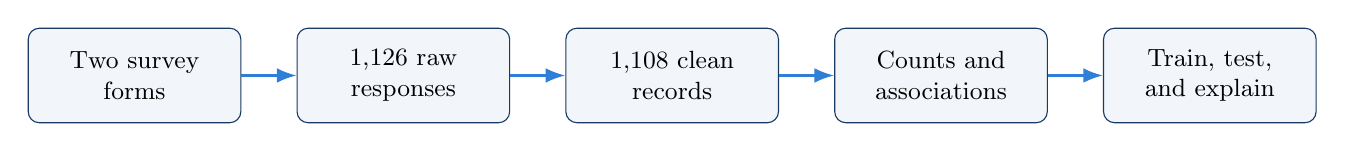
\begin{tikzpicture}[node distance=7mm, every node/.style={font=\small,align=center}, box/.style={draw=navy,rounded corners,minimum width=27mm,minimum height=12mm,fill=soft}, arr/.style={-{Latex[length=2.5mm]},thick,draw=blue}]
\node[box] (form) {Two survey\\forms};
\node[box,right=of form] (data) {1,126 raw\\responses};
\node[box,right=of data] (clean) {1,108 clean\\records};
\node[box,right=of clean] (desc) {Counts and\\associations};
\node[box,right=of desc] (ml) {Train, test,\\and explain};
\draw[arr] (form)--(data); \draw[arr] (data)--(clean); \draw[arr] (clean)--(desc); \draw[arr] (desc)--(ml);
\end{tikzpicture}
\caption{Project workflow from questionnaire collection to interpretable evaluation.}
\label{fig:project-flow}
\end{figure}


\section{Data description}
\subsection{Dataset overview}
The two source forms contain 1,126 responses. Target cleaning removes 18 rows without a usable CGPA response, giving 1,108 final records. Table~\ref{tab:composition} reports the institutional composition.

\begin{table}[H]\centering
\caption{Dataset composition after target cleaning.}\label{tab:composition}
\begin{tabular}{lrr}\toprule University&Records&Share (\%)\\\midrule
KUET&878&79.2\\BUET&104&9.4\\BRAC University&101&9.1\\CUET&25&2.3\\\midrule Total&1,108&100.0\\\bottomrule
\end{tabular}
\end{table}

\begin{figure}[H]\centering
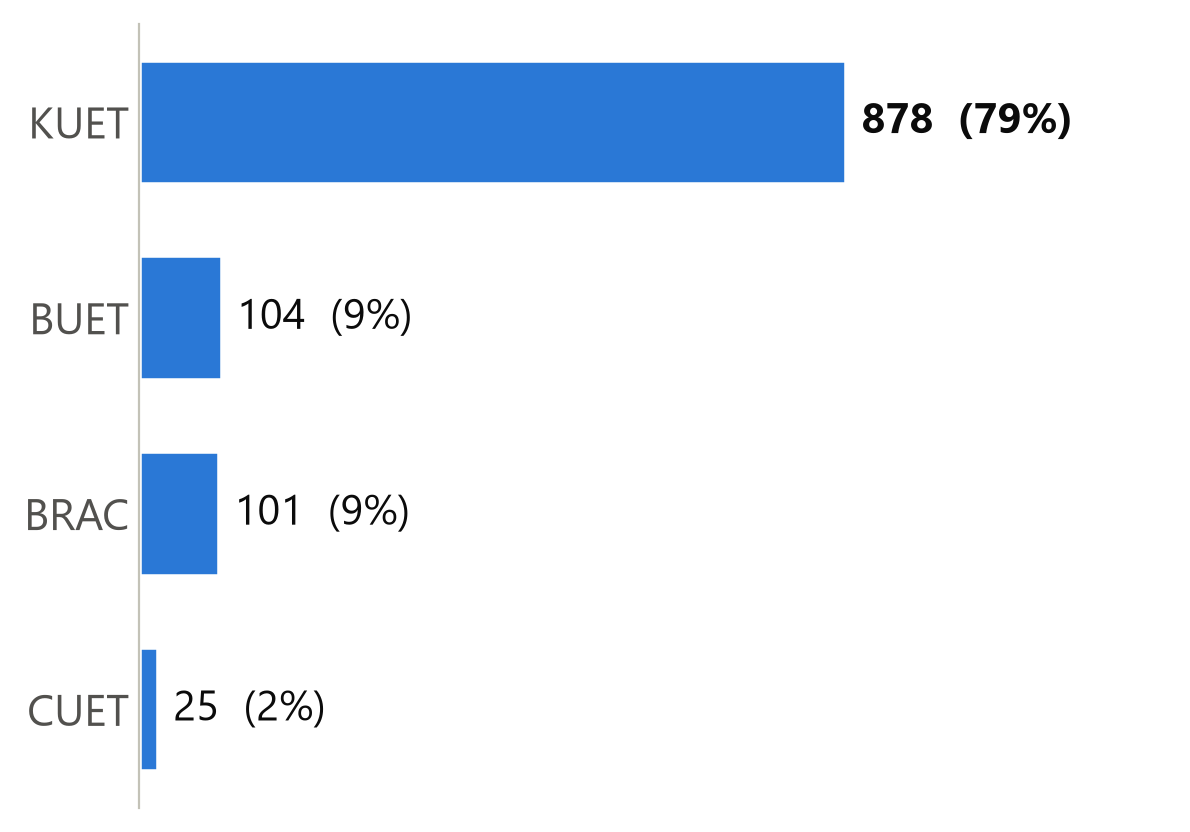
\includegraphics[width=0.84\textwidth]{figures/university_distribution.png}
\caption{University distribution in the cleaned dataset.}
\label{fig:university}
\end{figure}

\subsection{Questionnaire structure}
The common questionnaire covers academic context, study habits, lifestyle, pressure, motivation, support, environment, and grade outcomes. The two forms ask the same core questions but do not always use identical English text or answer formatting. Figure~\ref{fig:form} shows representative form content. No names or roll numbers appear in the modelling table.

\begin{figure}[H]\centering
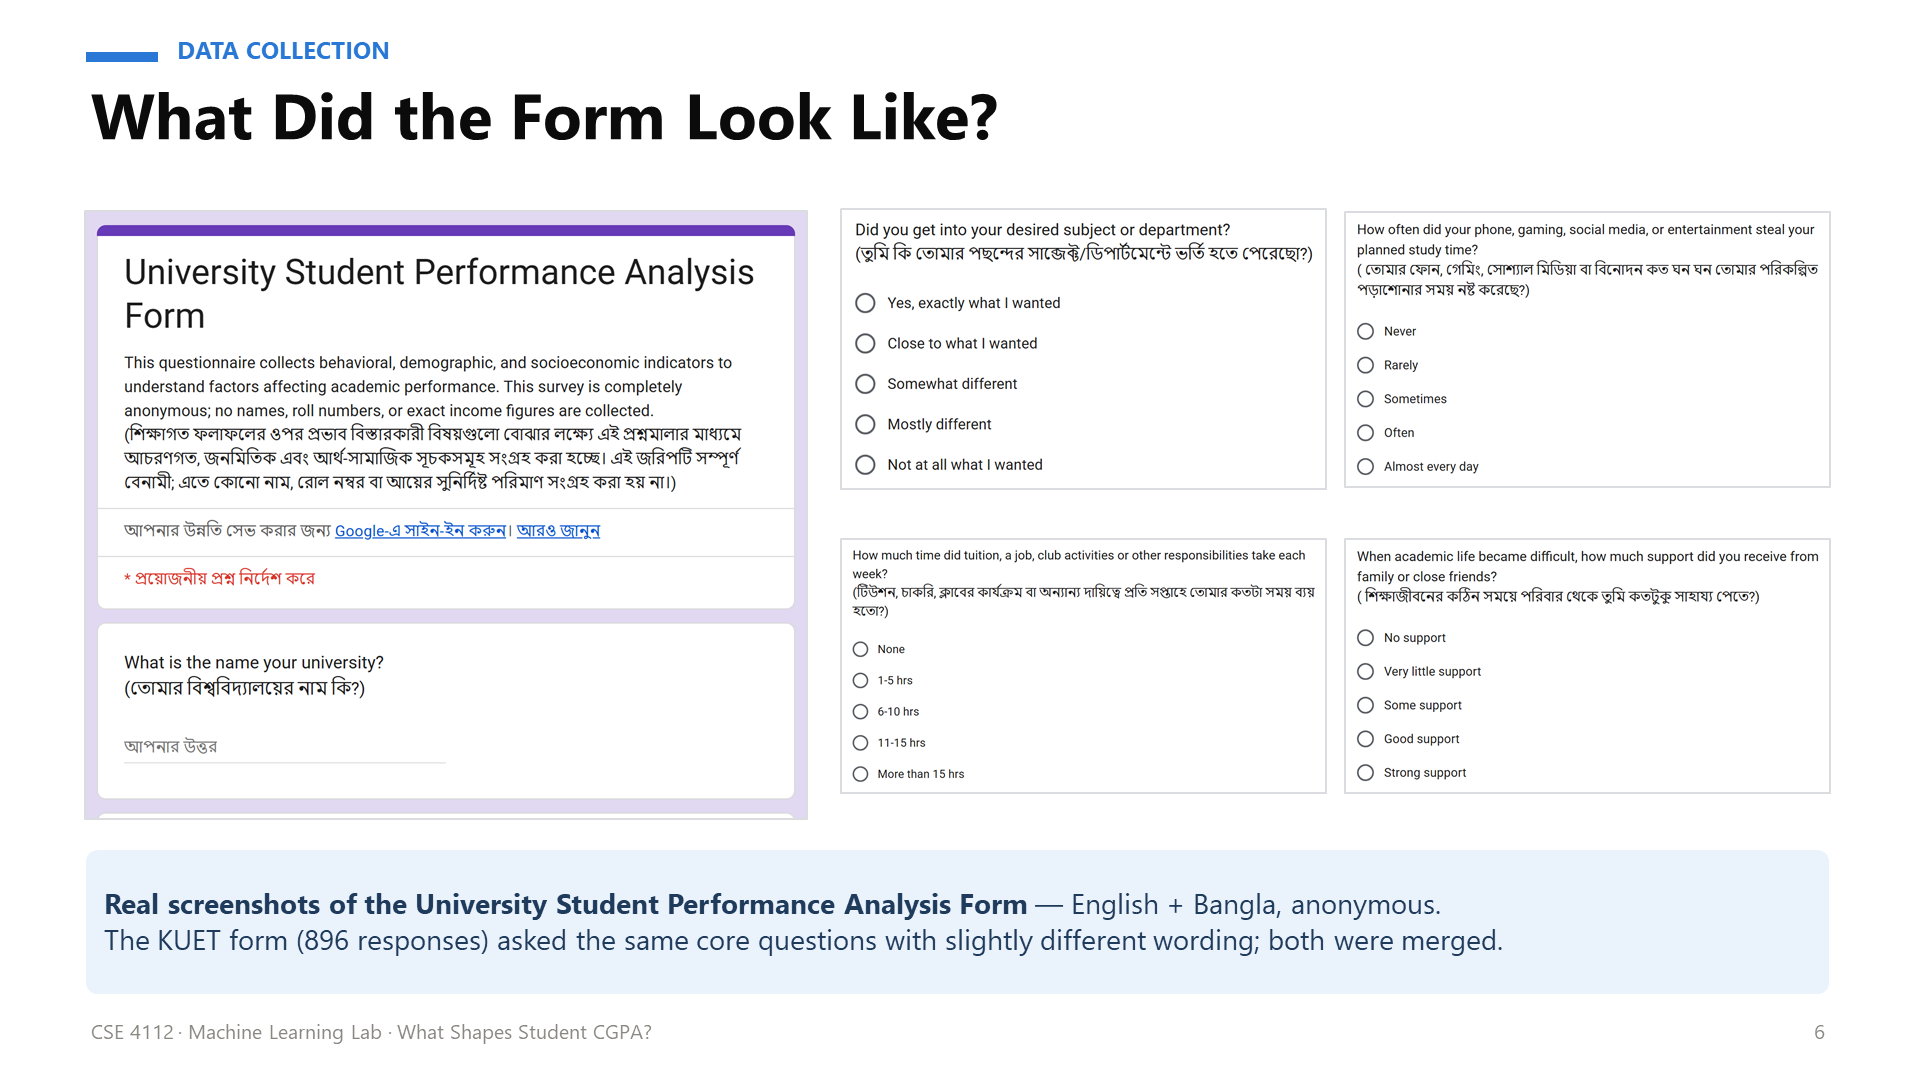
\includegraphics[width=0.95\textwidth]{figures/form_overview.png}
\caption{Representative form questions from the multi-university questionnaire. The KUET form used the same core concepts with some different wording.}
\label{fig:form}
\end{figure}

\begin{table}[H]\centering\small
\caption{Questionnaire variable groups.}\label{tab:variables}
\begin{tabularx}{\textwidth}{p{0.20\textwidth}Yp{0.24\textwidth}}\toprule
Group&Variables&Typical response form\\\midrule
Academic&University, department, semester, recent SGPA, CGPA&Nominal fields and ordered bands\\
Study habits&Attendance, weekly study time, study style, topic clarity&Five ordered categories\\
Lifestyle&Sleep duration, phone or social-media distraction&Five ordered categories\\
Pressure&Stress frequency, outside commitments&Frequency or hour bands\\
Motivation and support&Desired department, admission satisfaction, career expectation, family or friend support&Five ordered categories\\
Environment&Study-friendly living place, routine manageability&Five ordered categories\\\bottomrule
\end{tabularx}
\end{table}

\subsection{Response distributions}
All descriptive counts use the complete 1,108-row cleaned snapshot. For example, 418 students (37.7\%) report attendance of 90\% or more, 302 (27.3\%) report that stress sometimes blocks study, and 310 (28.0\%) report five to six hours of sleep. These figures describe answer frequencies only.

\begin{figure}[H]
\centering
\begin{subfigure}{0.49\textwidth}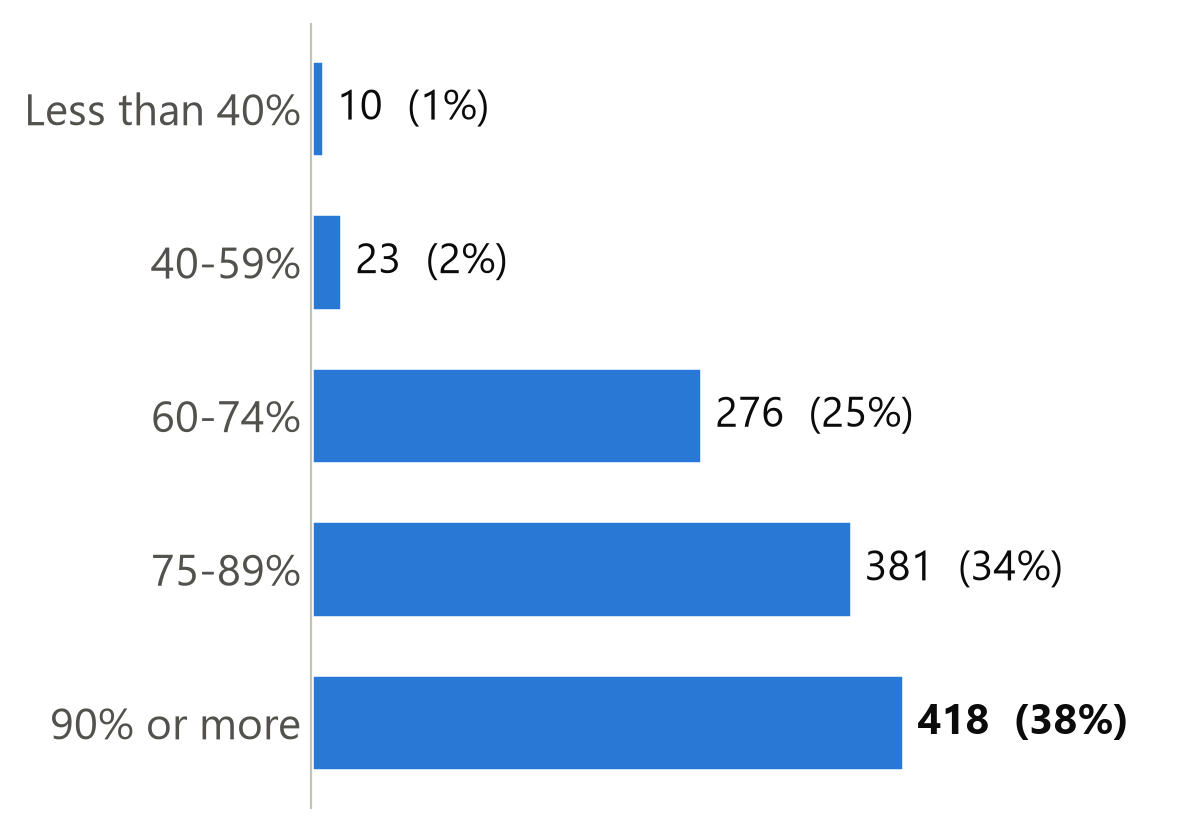
\includegraphics[width=\linewidth]{figures/attendance_distribution.png}\caption{Attendance}\end{subfigure}
\begin{subfigure}{0.49\textwidth}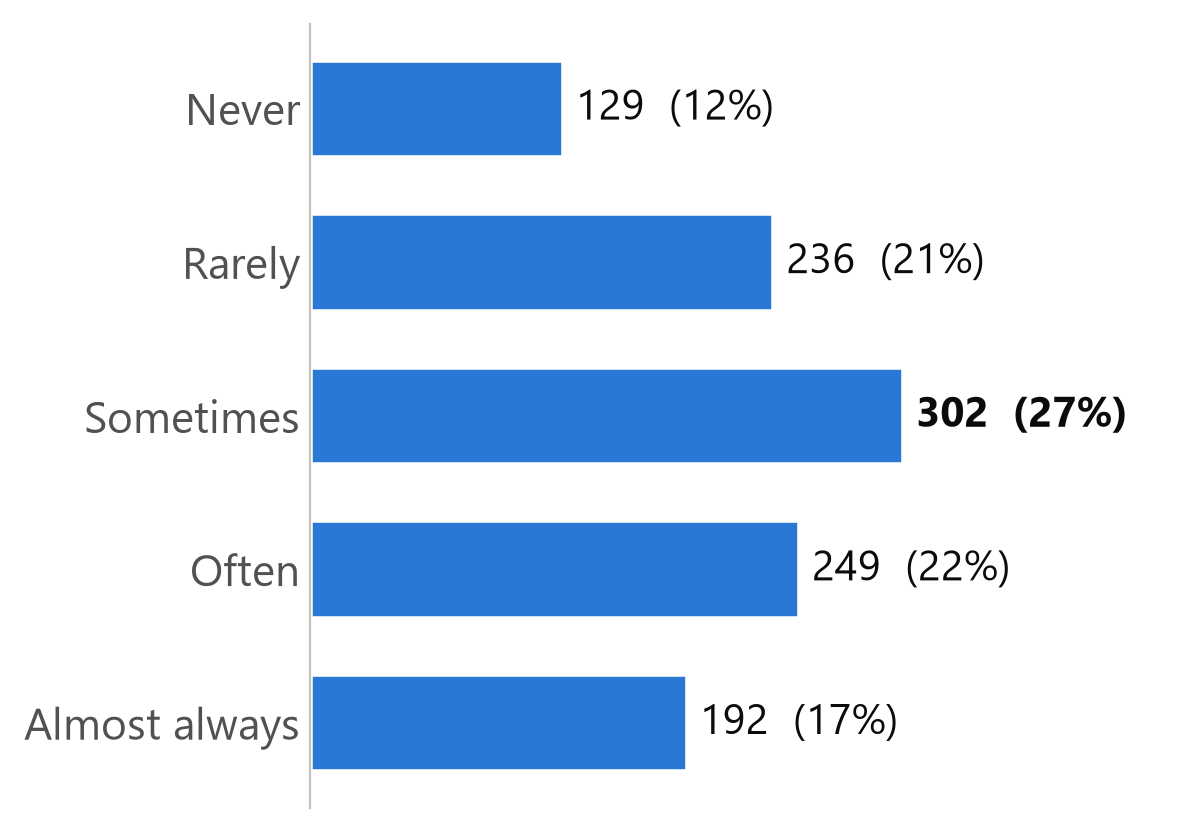
\includegraphics[width=\linewidth]{figures/stress_distribution.png}\caption{Stress frequency}\end{subfigure}
\caption{Examples of cleaned questionnaire response distributions.}
\label{fig:responses-a}
\end{figure}

\begin{figure}[H]\centering
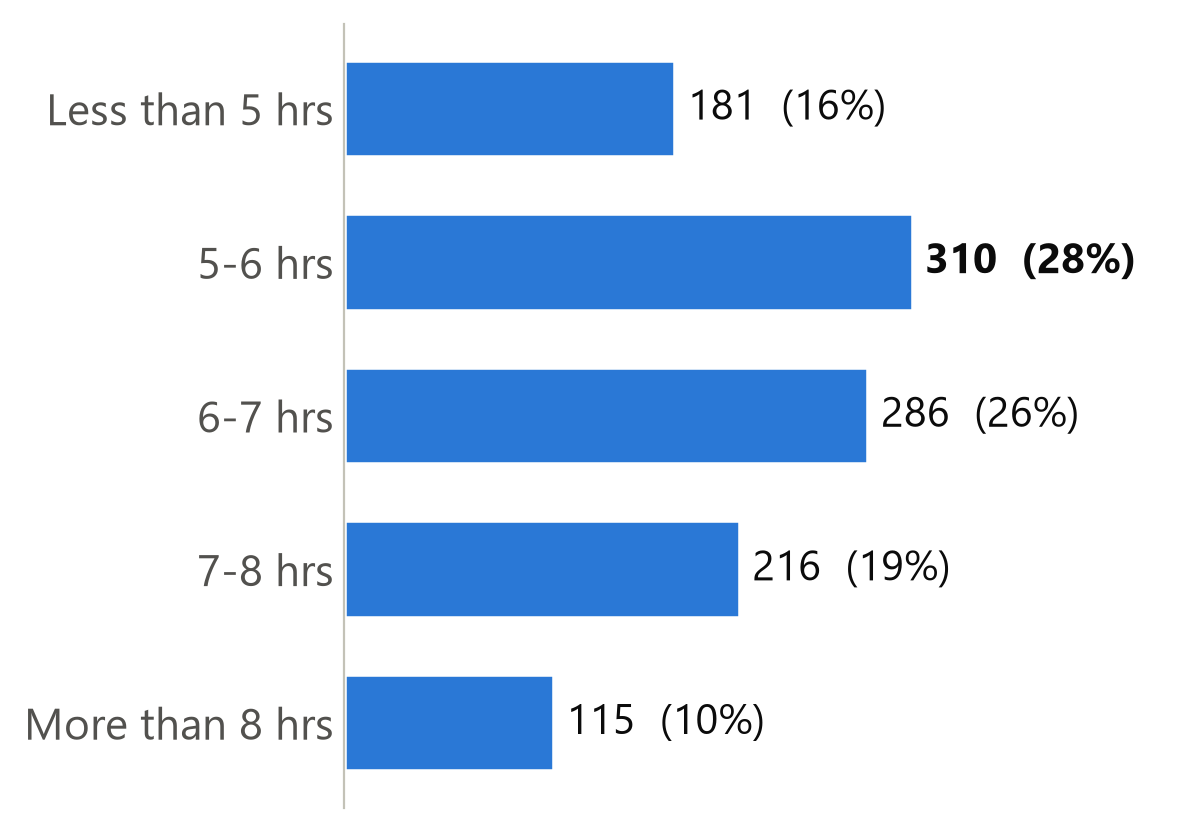
\includegraphics[width=0.72\textwidth]{figures/sleep_distribution.png}
\caption{Reported sleep duration in the cleaned dataset.}
\label{fig:sleep}
\end{figure}

\subsection{Target classes}
Both forms record grade ranges rather than a consistent exact numeric CGPA. The common target is therefore an ordered four-class variable.
\begin{table}[H]\centering
\caption{CGPA target groups.}\label{tab:classes}
\begin{tabular}{llrr}\toprule Code&CGPA range&Count&Share (\%)\\\midrule
C0&Below 3.20&236&21.3\\C1&3.20--3.49&321&29.0\\C2&3.50--3.74&303&27.3\\C3&3.75 and above&248&22.4\\\bottomrule
\end{tabular}
\end{table}
\begin{figure}[H]\centering
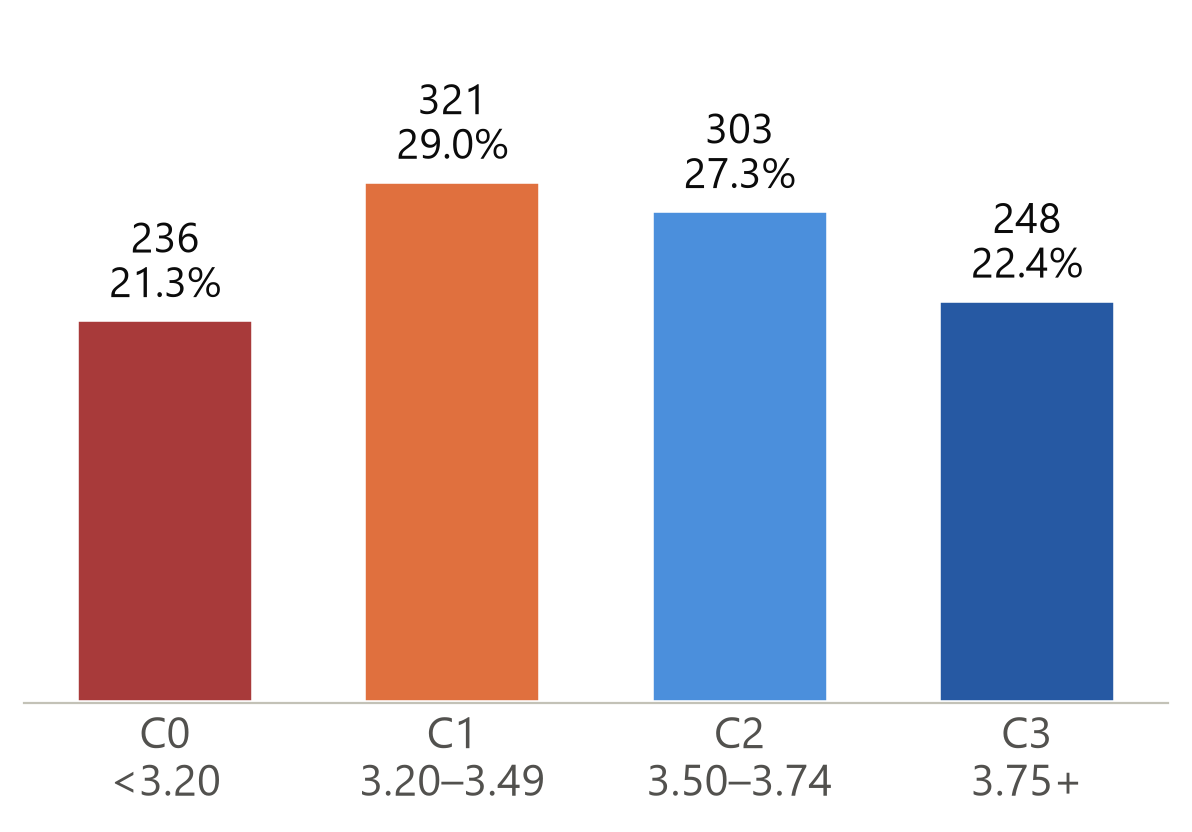
\includegraphics[width=0.72\textwidth]{figures/cgpa_distribution.png}
\caption{Distribution of the four CGPA target groups.}
\label{fig:cgpa-dist}
\end{figure}

\subsection{Reference dataset comparison}
The IUBAT reference dataset contains 894 Computer Science students and 31 columns, including exact numeric CGPA and SGPA, attendance, study hours, social-media hours, co-curricular activity, and socioeconomic variables \cite{prama2024}. The current questionnaire uses grade bands and adds direct questions about stress, sleep, topic clarity, desired department, support, study environment, and routine manageability.
\begin{figure}[H]\centering
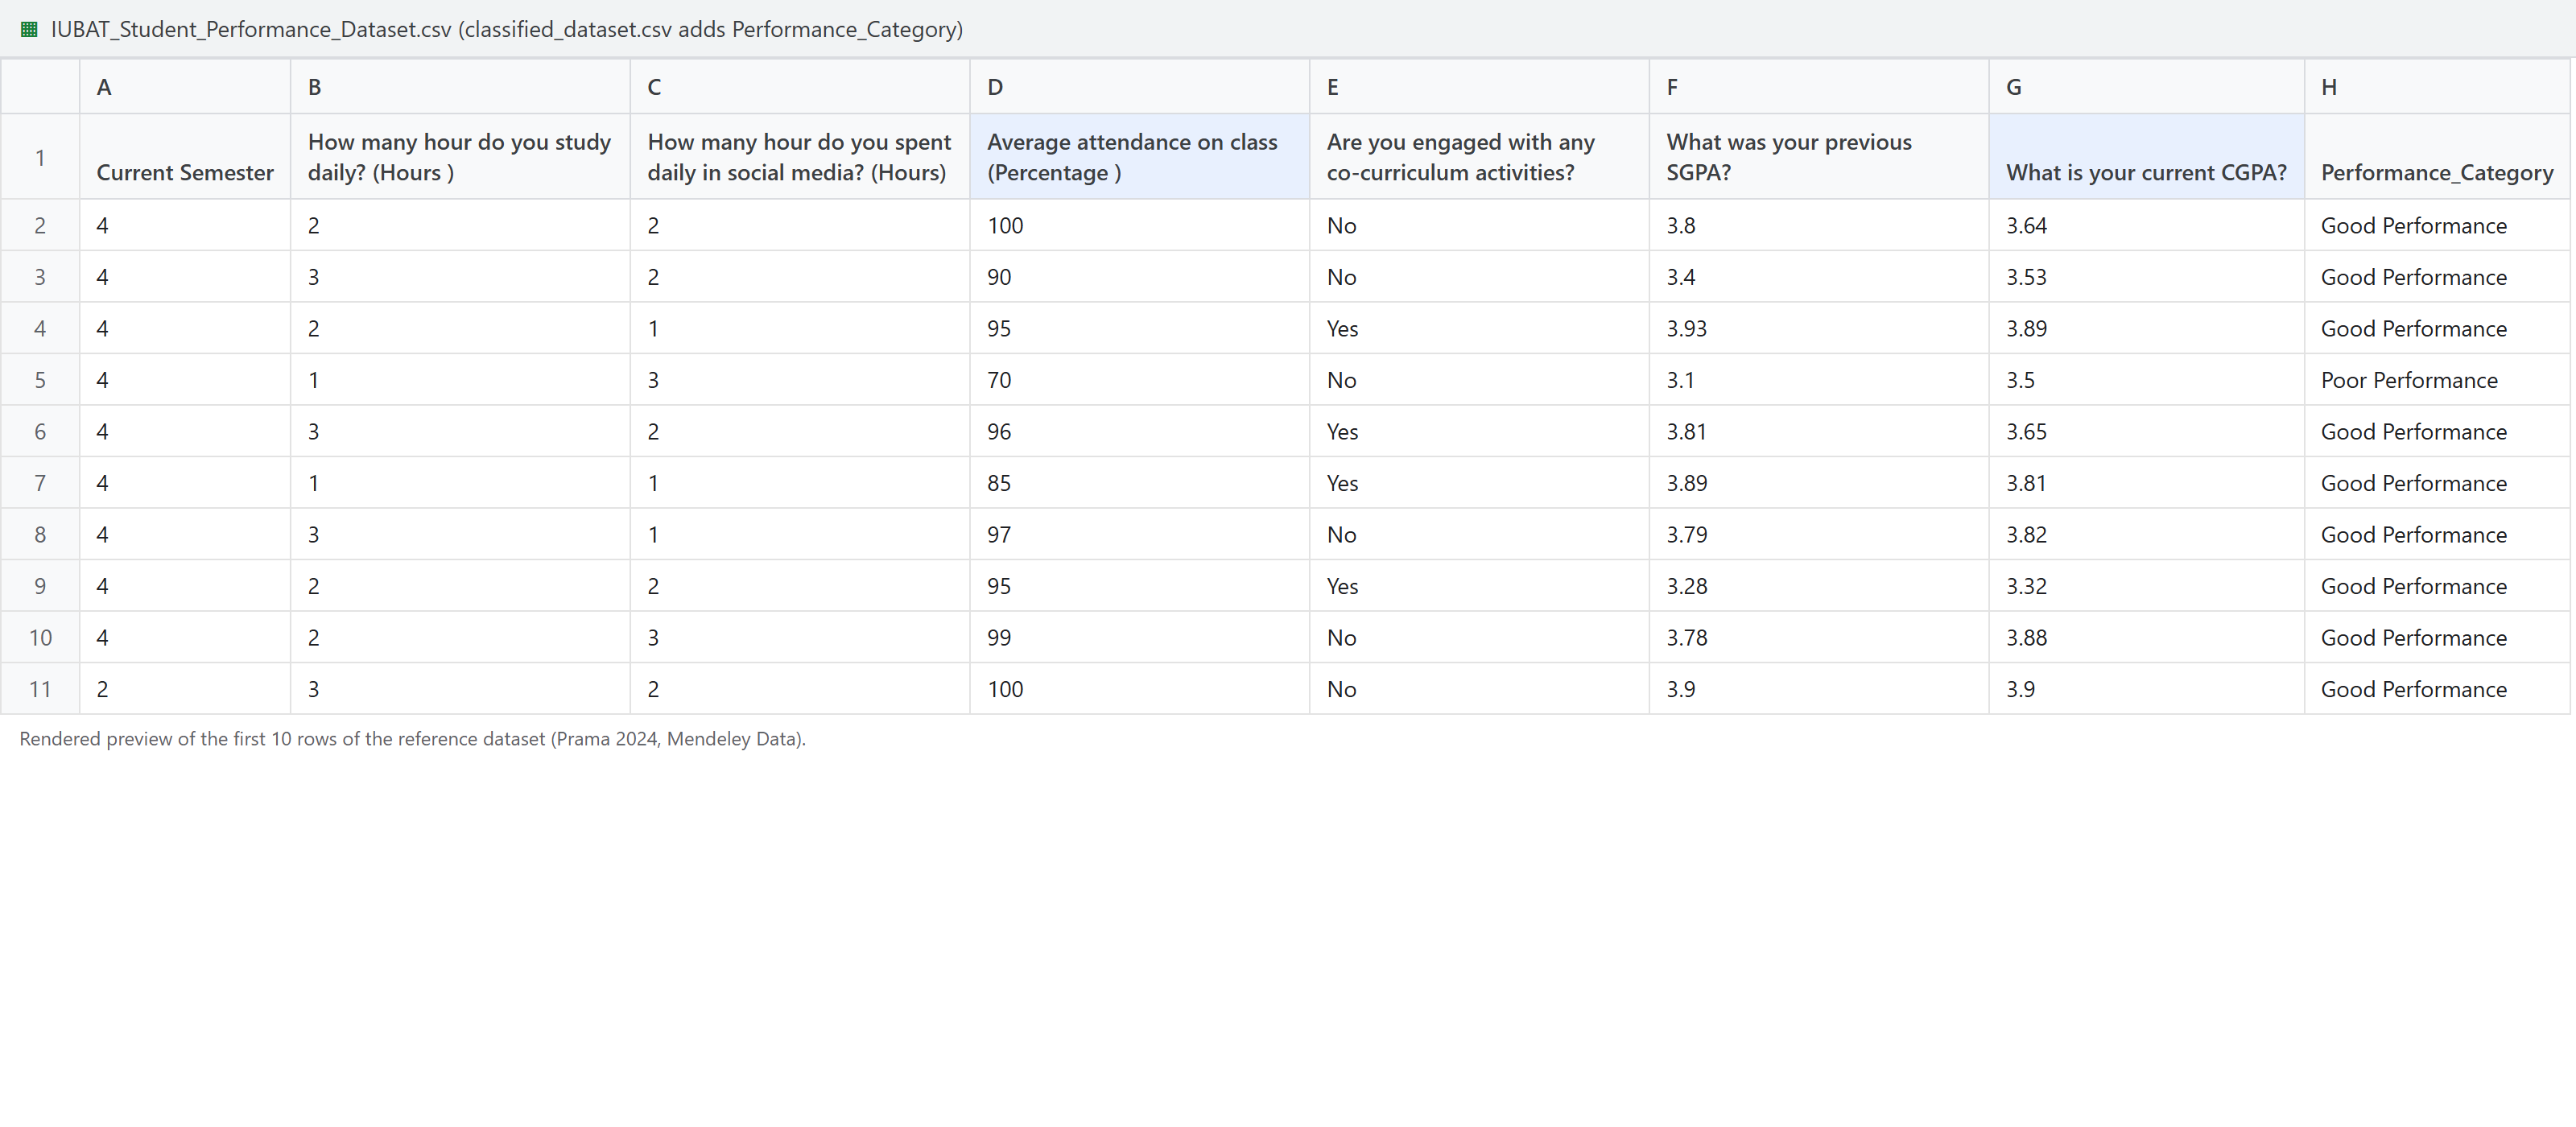
\includegraphics[width=0.95\textwidth]{figures/reference_dataset_preview.png}
\caption{Preview of the IUBAT reference dataset used to compare feature coverage.}
\label{fig:reference-preview}
\end{figure}

\subsection{Files and reproducibility}
The project package contains raw response files, three cleaned merged tables, WEKA-ready CSV and ARFF files, executed notebooks, machine-readable result summaries, figures, a data dictionary, cleaning logs, fixed split indices, and WEKA output logs. Figure~\ref{fig:dataset-preview} illustrates the cleaned row structure.
\begin{figure}[H]\centering
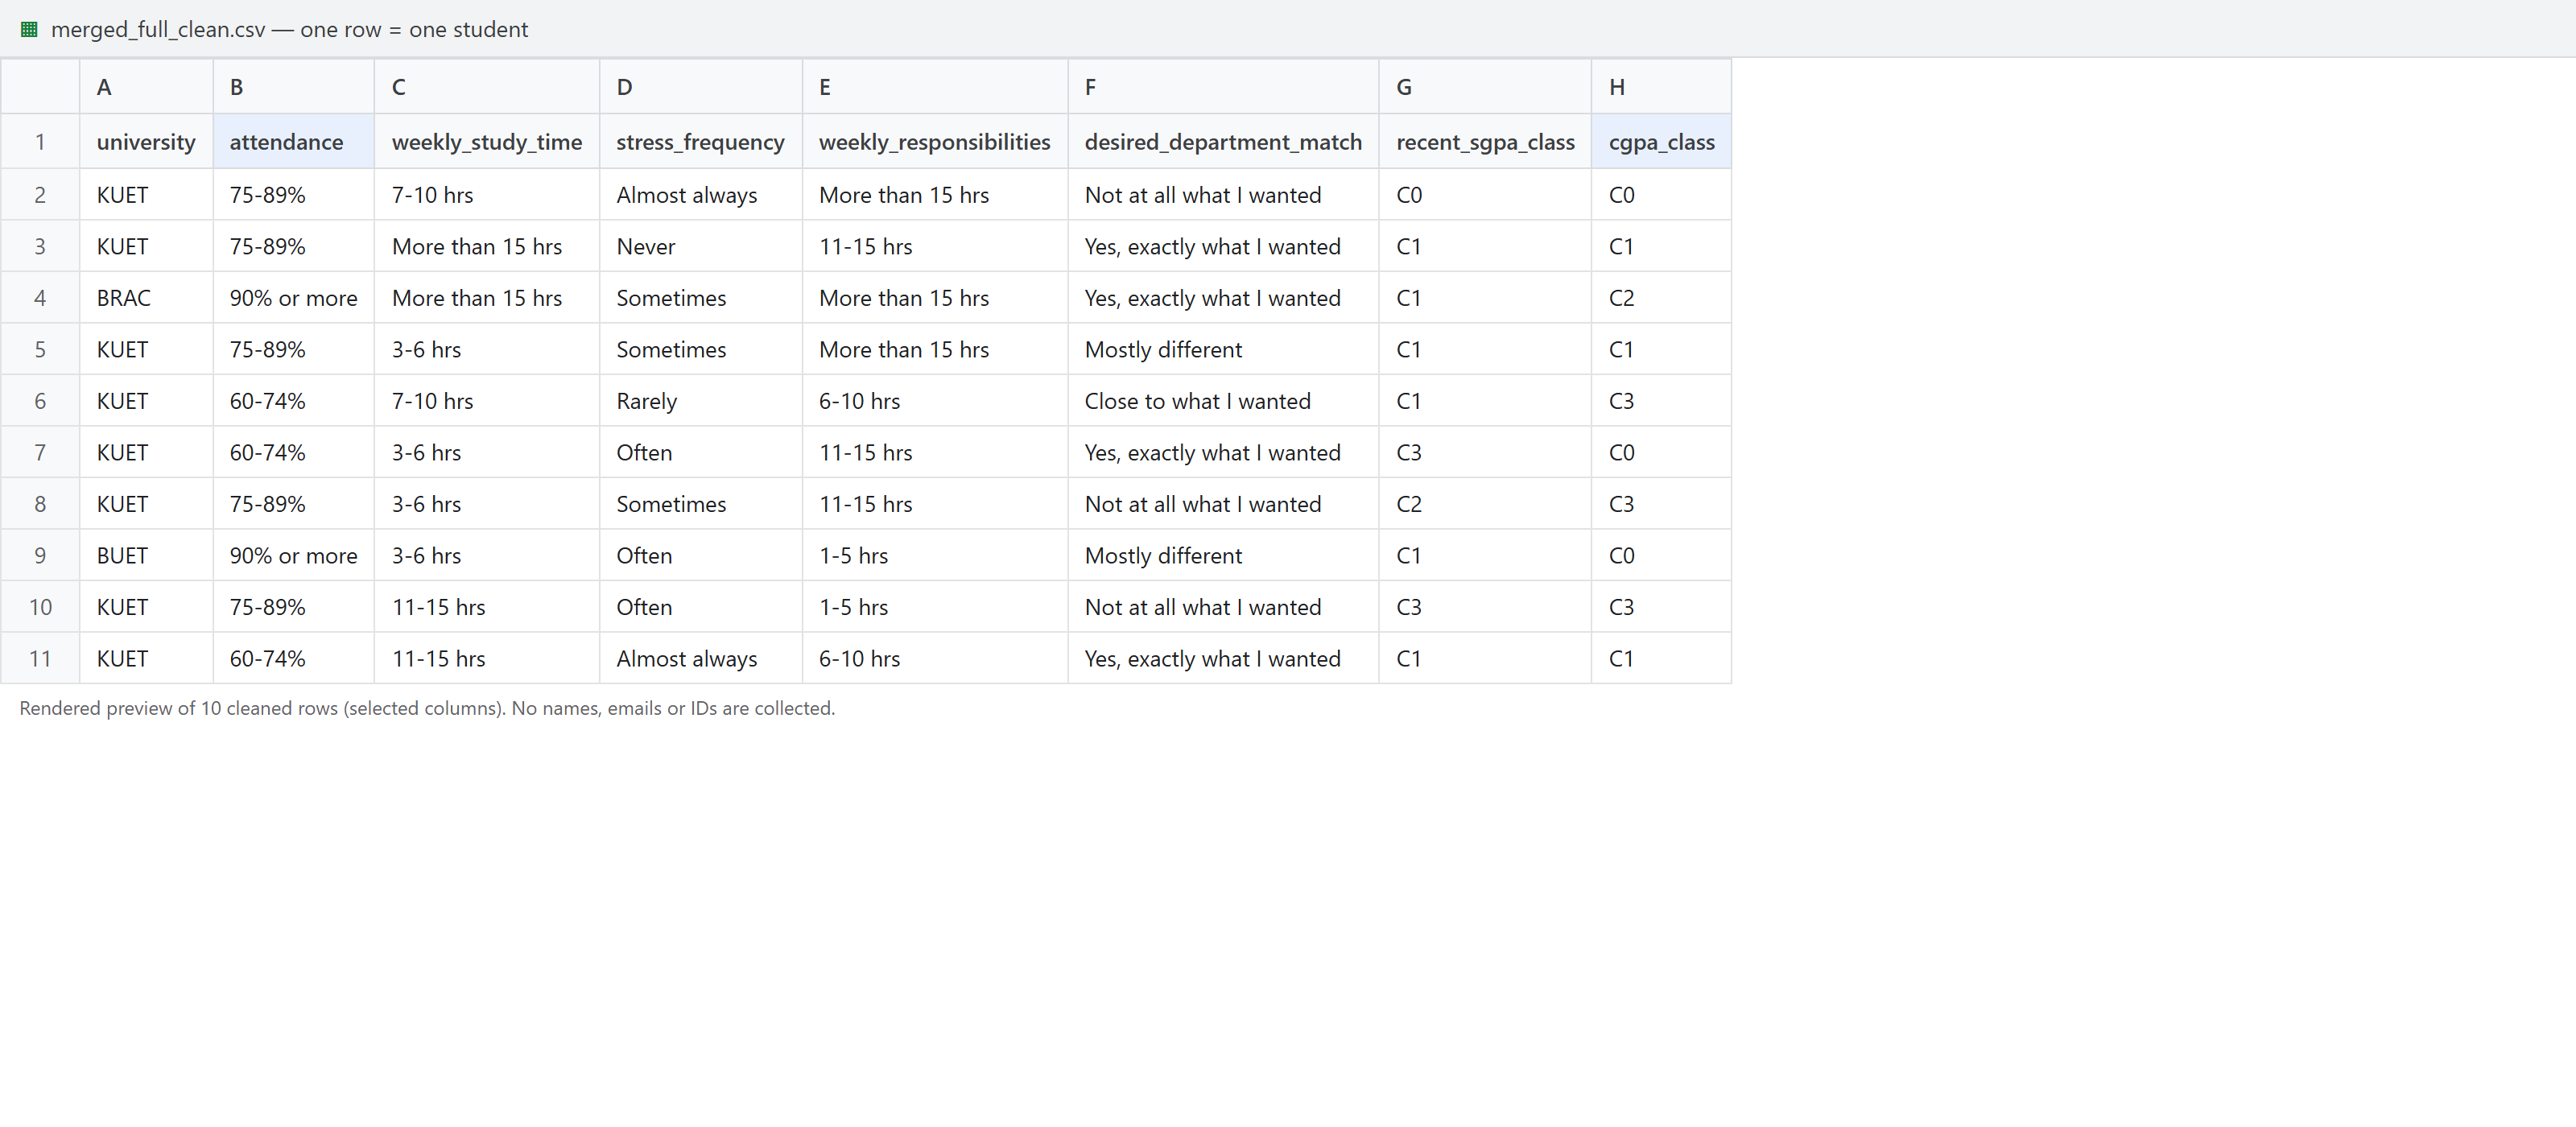
\includegraphics[width=0.95\textwidth]{figures/dataset_preview.png}
\caption{Cleaned dataset preview. One row represents one student response.}
\label{fig:dataset-preview}
\end{figure}


\section{Experimental design, materials, and methods}
\subsection{Questionnaire design and collection}
Two bilingual Google Forms collected responses from undergraduate engineering students. Source A contains 230 responses from BUET, BRAC University, and CUET. Source B contains 896 KUET responses. Both instruments cover 19 substantive concepts, while their column order, English phrasing, bilingual answer formatting, and grade-band options differ. The collection windows were 31 July to 13 August 2026 for the KUET form and 22 August to 3 September 2026 for the multi-university form.

\subsection{Schema mapping and harmonisation}
Each raw column was mapped by hand to a common \code{snake\_case} schema and guarded by assertions. Manual mapping was selected because automatic text similarity could incorrectly merge conceptually different satisfaction questions. The harmonisation pass removed emoji and Bangla parenthetical translations from answer values while preserving English department abbreviations. One study-style label was reconciled, and the two grade-band schemes plus typed KUET values were mapped into C0--C3.

The pipeline retained a source-form field for audit comparisons but excluded it from modelling. It dropped timestamps because the collection windows identify the source form, and it removed an empty email column. University spelling variants were reduced to four institutions. A rule-based canonicaliser reduced 110 free-text department strings to 24 department names, then grouped categories with fewer than 15 students for modelling.

\subsection{Cleaning sequence}
\begin{table}[H]\centering\small
\caption{Auditable cleaning sequence.}\label{tab:cleaning}
\begin{tabularx}{\textwidth}{p{0.08\textwidth}p{0.35\textwidth}Yp{0.11\textwidth}}\toprule
Step&Decision&Reason&Rows\\\midrule
1&Drop timestamp&Collection timing is a source proxy, not a student attribute&1,126\\
2&Normalise 10 university labels to 4&Case and suffix variants identify the same institution&1,126\\
3&Canonicalise 110 department strings to 24&Abbreviations, spelling, and free text otherwise split categories&1,126\\
4&Reconcile one study-style label&Keep the ordered scale consistent across forms&1,126\\
5&Build four CGPA groups&Four classes are recoverable from both questionnaires&1,126\\
6&Remove unusable CGPA targets&A supervised model cannot learn from an unlabelled target&1,108\\
7&Map supported commitment blanks to None&The KUET form provides an explicit None option with a comparable response rate&1,108\\
8&Fill remaining sparse predictor blanks&Within-source modal categories preserve the observed category labels&1,108\\
9&Encode ordered scales&Preserve the natural order of the responses&1,108\\
10&Derive academic progress and audit features&Replace raw semester with a comparable progress measure&1,108\\\bottomrule
\end{tabularx}
\end{table}

\subsection{Missing values and leakage control}
Only 18 rows were removed, all because their CGPA target could not be interpreted. Blank outside-commitment answers were handled as None when the form design and response rates supported that meaning. The remaining predictor missingness was below 1.3\% per field and was filled with the modal category from the same source form. Six rows had recent SGPA filled using information from their CGPA class in the earlier cleaning process. Descriptive summaries retain those rows, but every final model experiment excludes them. The resulting modelling set contains 1,102 students.

Result satisfaction was omitted from predictive feature sets because it follows an academic outcome. Source form was also excluded so the model could not learn questionnaire identity. University, department, and raw semester were not used in the 12-question teacher-facing trees.

\subsection{Data quality checks}
Quality checks covered class balance, source-form option overlap, university imbalance, duplicates, category coverage, missingness, and complete-case sensitivity. In the 1,108-row descriptive snapshot, target shares range from 21.3\% to 29.0\%. After the six-row modelling exclusion, the CGPA ZeroR baseline is 29.04\% in 10-fold cross-validation. KUET contributes 79.2\% of cleaned records and therefore requires an explicit generalisation warning. Complete-case recalculation changed no reported Spearman coefficient by more than 0.0036.

\begin{figure}[H]\centering
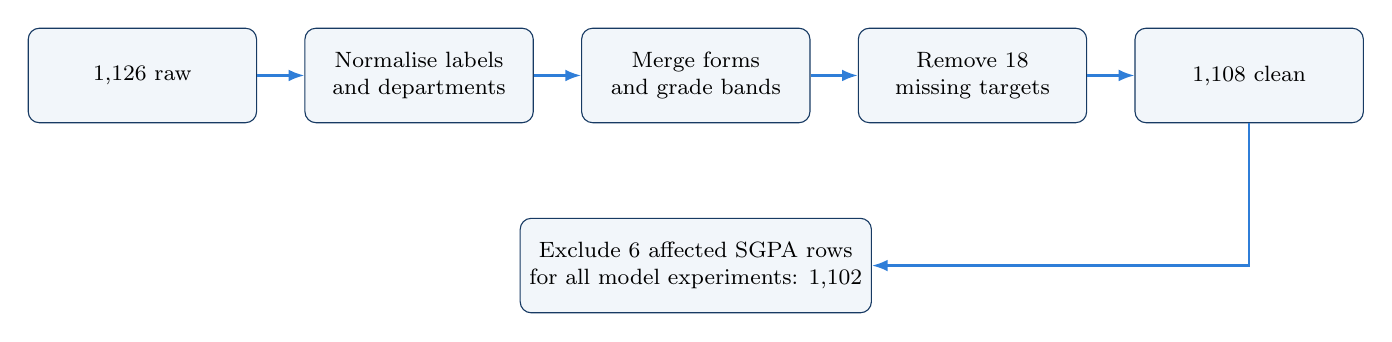
\begin{tikzpicture}[node distance=6mm, every node/.style={font=\footnotesize,align=center}, p/.style={draw=navy,fill=soft,rounded corners,minimum width=29mm,minimum height=12mm}, a/.style={-{Latex[length=2mm]},thick,draw=blue}]
\node[p] (raw) {1,126 raw};
\node[p,right=of raw] (labels) {Normalise labels\\and departments};
\node[p,right=of labels] (merge) {Merge forms\\and grade bands};
\node[p,right=of merge] (drop) {Remove 18\\missing targets};
\node[p,right=of drop] (clean) {1,108 clean};
\draw[a] (raw)--(labels);\draw[a] (labels)--(merge);\draw[a] (merge)--(drop);\draw[a] (drop)--(clean);
\node[p,below=12mm of merge] (tree) {Exclude 6 affected SGPA rows\\for all model experiments: 1,102};
\draw[a] (clean.south) |- (tree.east);
\end{tikzpicture}
\caption{Cleaning and teacher-facing experiment populations.}
\label{fig:cleaning-flow}
\end{figure}

\section{Data limitations}
\begin{itemize}
\item Grades and behaviours are self-reported and were not checked against registrar records.
\item The convenience sample is dominated by KUET, which contributes 79.2\% of the records.
\item The survey is cross-sectional. It measures each student once and cannot observe changes across semesters.
\item CGPA and SGPA are stored as bands rather than consistent exact numbers.
\item Small wording and option differences remain between the two questionnaires after semantic harmonisation.
\item Source A asks for CGPA before the most recent semester, while Source B asks for current CGPA. This one-semester reference difference affects interpretation of the SGPA feature.
\item The dataset does not contain verified course-level grades, longitudinal activity, or equally sized samples from all universities.
\item Questionnaire missing-value modes were calculated before cross-validation and before the fixed train/test split. This historical preprocessing order can transfer limited distribution information into evaluation data.
\end{itemize}
These limitations restrict population-level generalisation and any intended high-stakes use. The model scores are exploratory course-project evidence. They remain useful for reproducible classroom analysis when the sampling, measurement, and preprocessing boundaries stay visible.


\partbanner{Part II: Machine Learning Analysis}
\section{Machine-learning analysis framework}
\subsection{Research questions}
\begin{enumerate}
\item Which questionnaire variables show the clearest descriptive relationship with CGPA groups?
\item Can the 12 questionnaire variables predict recent SGPA or CGPA for an unseen student?
\item How much predictive structure appears when recent SGPA is added to the CGPA inputs?
\item Which rules appear in a readable WEKA J48 tree, and how does that tree behave on the fixed test set?
\end{enumerate}

\subsection{Feature sets and targets}
Three separate four-class tasks were prepared. Recent SGPA prediction uses 12 questionnaire variables: attendance, weekly study time, study style, topic clarity, sleep, stress, outside commitments, digital distraction, study environment, support, desired-department match, and routine manageability. The questionnaire-only CGPA task uses the same 12 inputs. The main CGPA task adds recent SGPA as a thirteenth input. The ordered classes are C0, C1, C2, and C3.

All descriptive summaries use 1,108 cleaned records. Every model uses 1,102 records after excluding six rows whose recent SGPA had previously been imputed using the CGPA class. University, department, semester, source form, identifiers, and result satisfaction are excluded from all three feature sets.

\subsection{Two WEKA evaluation views}
The model comparison uses stratified 10-fold cross-validation on all 1,102 eligible records with seed 1. J48, Random Forest, SMO, Logistic, Naive Bayes, and ZeroR are run on each of the three tasks under the same evaluation protocol.

The explanatory tree view uses the existing CGPA-stratified split with seed 42: 881 training rows and 221 test rows. The identical row indices are reused for all three targets. WEKA J48 uses confidence factor 0.25 and minimum leaf size 40 so that its exact tree is readable. The setting was specified for explanation rather than selected from test accuracy. ZeroR is fitted on the training rows and evaluated on the same test rows.

\begin{figure}[H]\centering
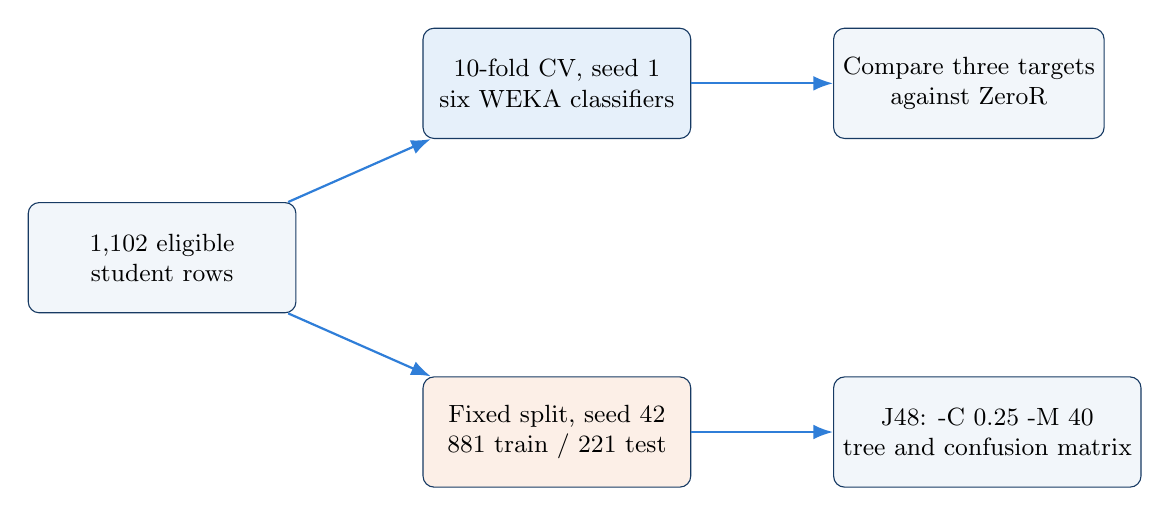
\begin{tikzpicture}[node distance=7mm, every node/.style={font=\small,align=center}, b/.style={draw=navy,rounded corners,fill=soft,minimum width=34mm,minimum height=14mm}, a/.style={-{Latex[length=2.5mm]},thick,draw=blue}]
\node[b] (eligible) {1,102 eligible\\student rows};
\node[b,above right=8mm and 16mm of eligible,fill=blue!12] (cv) {10-fold CV, seed 1\\six WEKA classifiers};
\node[b,right=18mm of cv] (compare) {Compare three targets\\against ZeroR};
\node[b,below right=8mm and 16mm of eligible,fill=orange!12] (split) {Fixed split, seed 42\\881 train / 221 test};
\node[b,right=18mm of split] (tree) {J48: -C 0.25 -M 40\\tree and confusion matrix};
\draw[a] (eligible)--(cv);\draw[a] (cv)--(compare);
\draw[a] (eligible)--(split);\draw[a] (split)--(tree);
\end{tikzpicture}
\caption{The WEKA model comparison and explanatory J48 evaluation use separately labelled protocols.}
\label{fig:evaluation-flow}
\end{figure}

\subsection{Preprocessing boundary}
The raw-to-clean verification was re-executed before the final WEKA run and reproduced every modelling column used in the ARFF files. Questionnaire missing-value modes, however, were calculated in the historical cleaning pipeline before cross-validation and before the fixed split. This can transfer limited distribution information across folds. The reported scores are therefore exploratory course-project estimates rather than deployment estimates.

\begin{table}[H]\centering
\caption{Final WEKA prediction tasks.}\label{tab:tree-tasks}
\begin{tabularx}{\textwidth}{p{0.27\textwidth}p{0.32\textwidth}Y}\toprule
Prediction target&Inputs&Purpose\\\midrule
Recent SGPA&12 questionnaire answers&Test the predictive signal for recent academic performance\\
CGPA questionnaire-only&12 questionnaire answers&Measure how far survey responses alone rise above the CGPA baseline\\
Main CGPA&12 answers plus recent SGPA&Measure the strongest available CGPA task and inspect its readable rules\\\bottomrule
\end{tabularx}
\end{table}

\section{Models and evaluation}
\subsection{Models}
The final comparison uses six WEKA 3.8.7 classifiers \cite{weka2009}. J48 supplies a readable decision tree. Random Forest supplies a non-linear ensemble benchmark. SMO supplies the course-tool support-vector-machine implementation. Logistic Regression gives a linear classifier, Naive Bayes gives a probabilistic comparison, and ZeroR predicts only the majority class.

The 10-fold J48 run uses confidence factor 0.25 and WEKA's default minimum leaf size of 2. Random Forest uses 100 trees and seed 1. The explanatory fixed-split J48 uses confidence factor 0.25 and minimum leaf size 40. This larger leaf size keeps the exact WEKA tree readable. The cross-validation J48 and the fixed-split J48 answer different questions and are reported separately.

\subsection{Metrics}
\begin{table}[H]\centering
\caption{Evaluation measures and interpretation.}\label{tab:metrics}
\begin{tabularx}{\textwidth}{p{0.24\textwidth}Y}\toprule
Measure&Role\\\midrule
Exact accuracy&Primary fraction of students assigned to the correct group\\
Weighted F1&Frequency-weighted class performance reported by WEKA\\
Cohen's kappa&Agreement after accounting for chance\\
Confusion matrix&Counts for every actual and predicted group\\
Absolute class distance&Ordinal error magnitude: 0 exact, 1 adjacent, 2 or 3 farther away\\\bottomrule
\end{tabularx}
\end{table}

The majority baseline depends on the target and evaluation subset. In 10-fold cross-validation, ZeroR reaches 26.86\% for recent SGPA and 29.04\% for both CGPA tasks. On the 221-row fixed test set, ZeroR reaches 27.15\% for recent SGPA and 28.96\% for both CGPA tasks. Scores close to those values require cautious interpretation.

\section{Results}
\subsection{Descriptive CGPA patterns}
Three questionnaire variables show the clearest corrected association with CGPA: desired-department match ($\rho=+0.119$, adjusted $q=0.0010$), attendance ($\rho=+0.090$, $q=0.0197$), and outside commitments ($\rho=-0.086$, $q=0.0202$). Each association is small. Figures~\ref{fig:attendance-cgpa}--\ref{fig:department-cgpa} show group composition rather than causal effects.

\begin{figure}[H]\centering
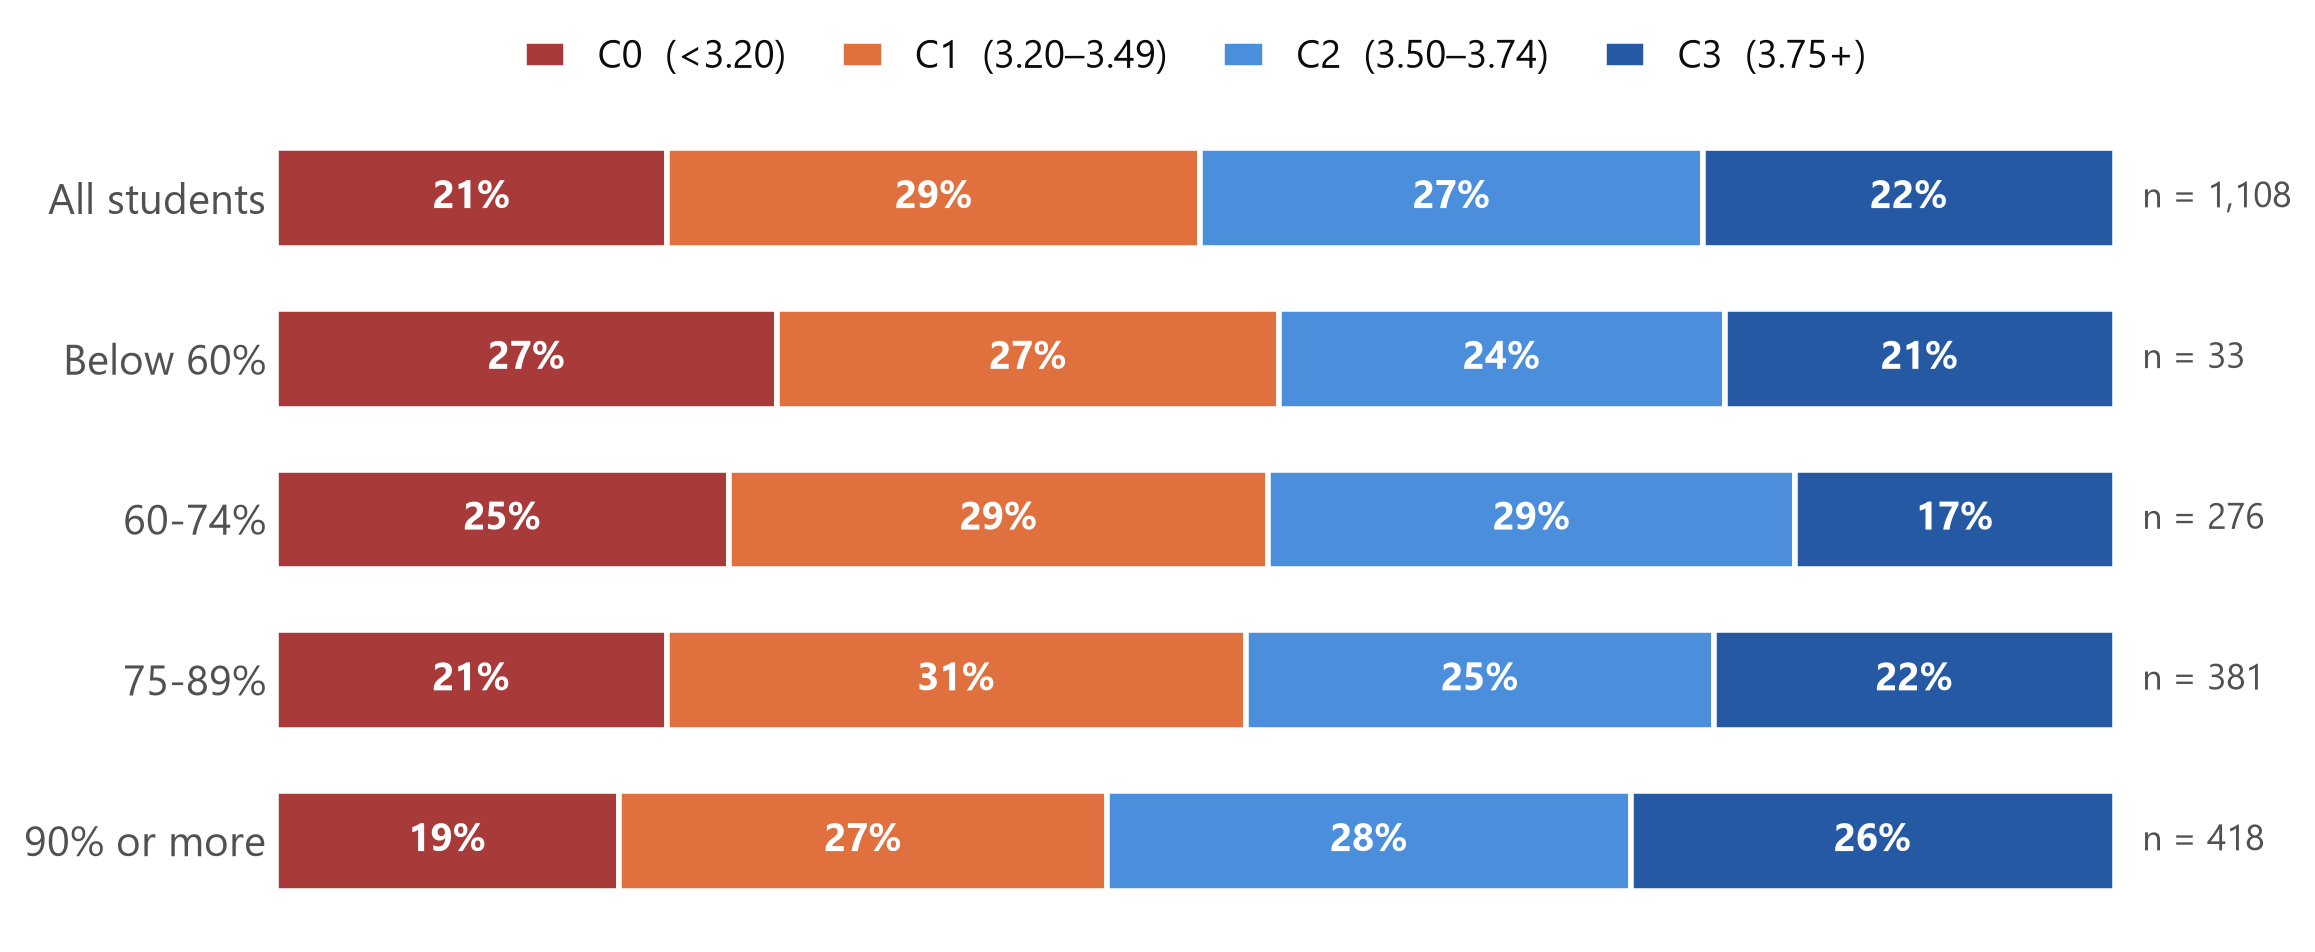
\includegraphics[width=0.9\textwidth]{figures/attendance_cgpa.png}
\caption{CGPA-group composition by attendance band. Students reporting 90\% or more attendance have a 55\% C2/C3 share, compared with 46\% for the 60--74\% group.}
\label{fig:attendance-cgpa}
\end{figure}

\begin{figure}[H]\centering
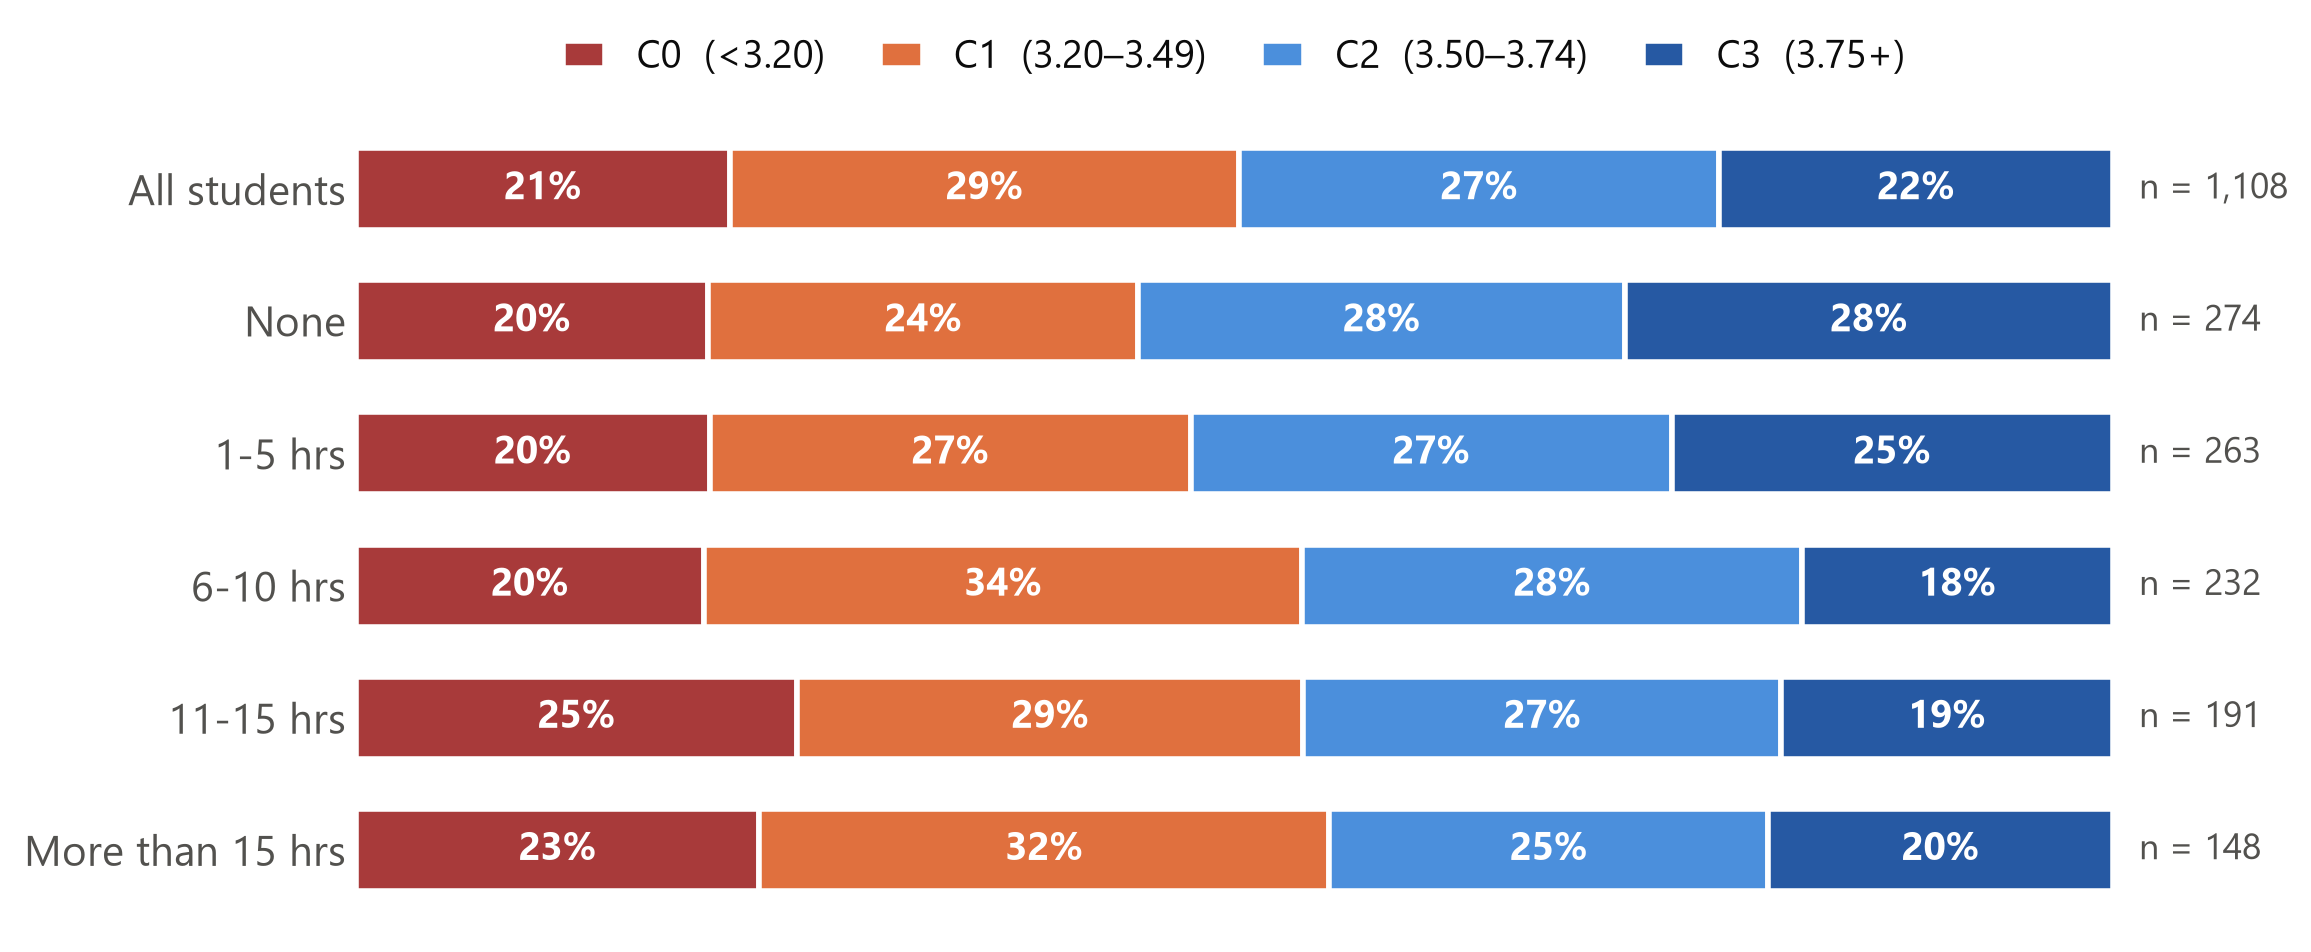
\includegraphics[width=0.9\textwidth]{figures/commitments_cgpa.png}
\caption{CGPA-group composition by weekly outside commitments. The C2/C3 share is 56\% for no outside commitments and 45\% above 15 hours.}
\label{fig:commitments-cgpa}
\end{figure}

\begin{figure}[H]\centering
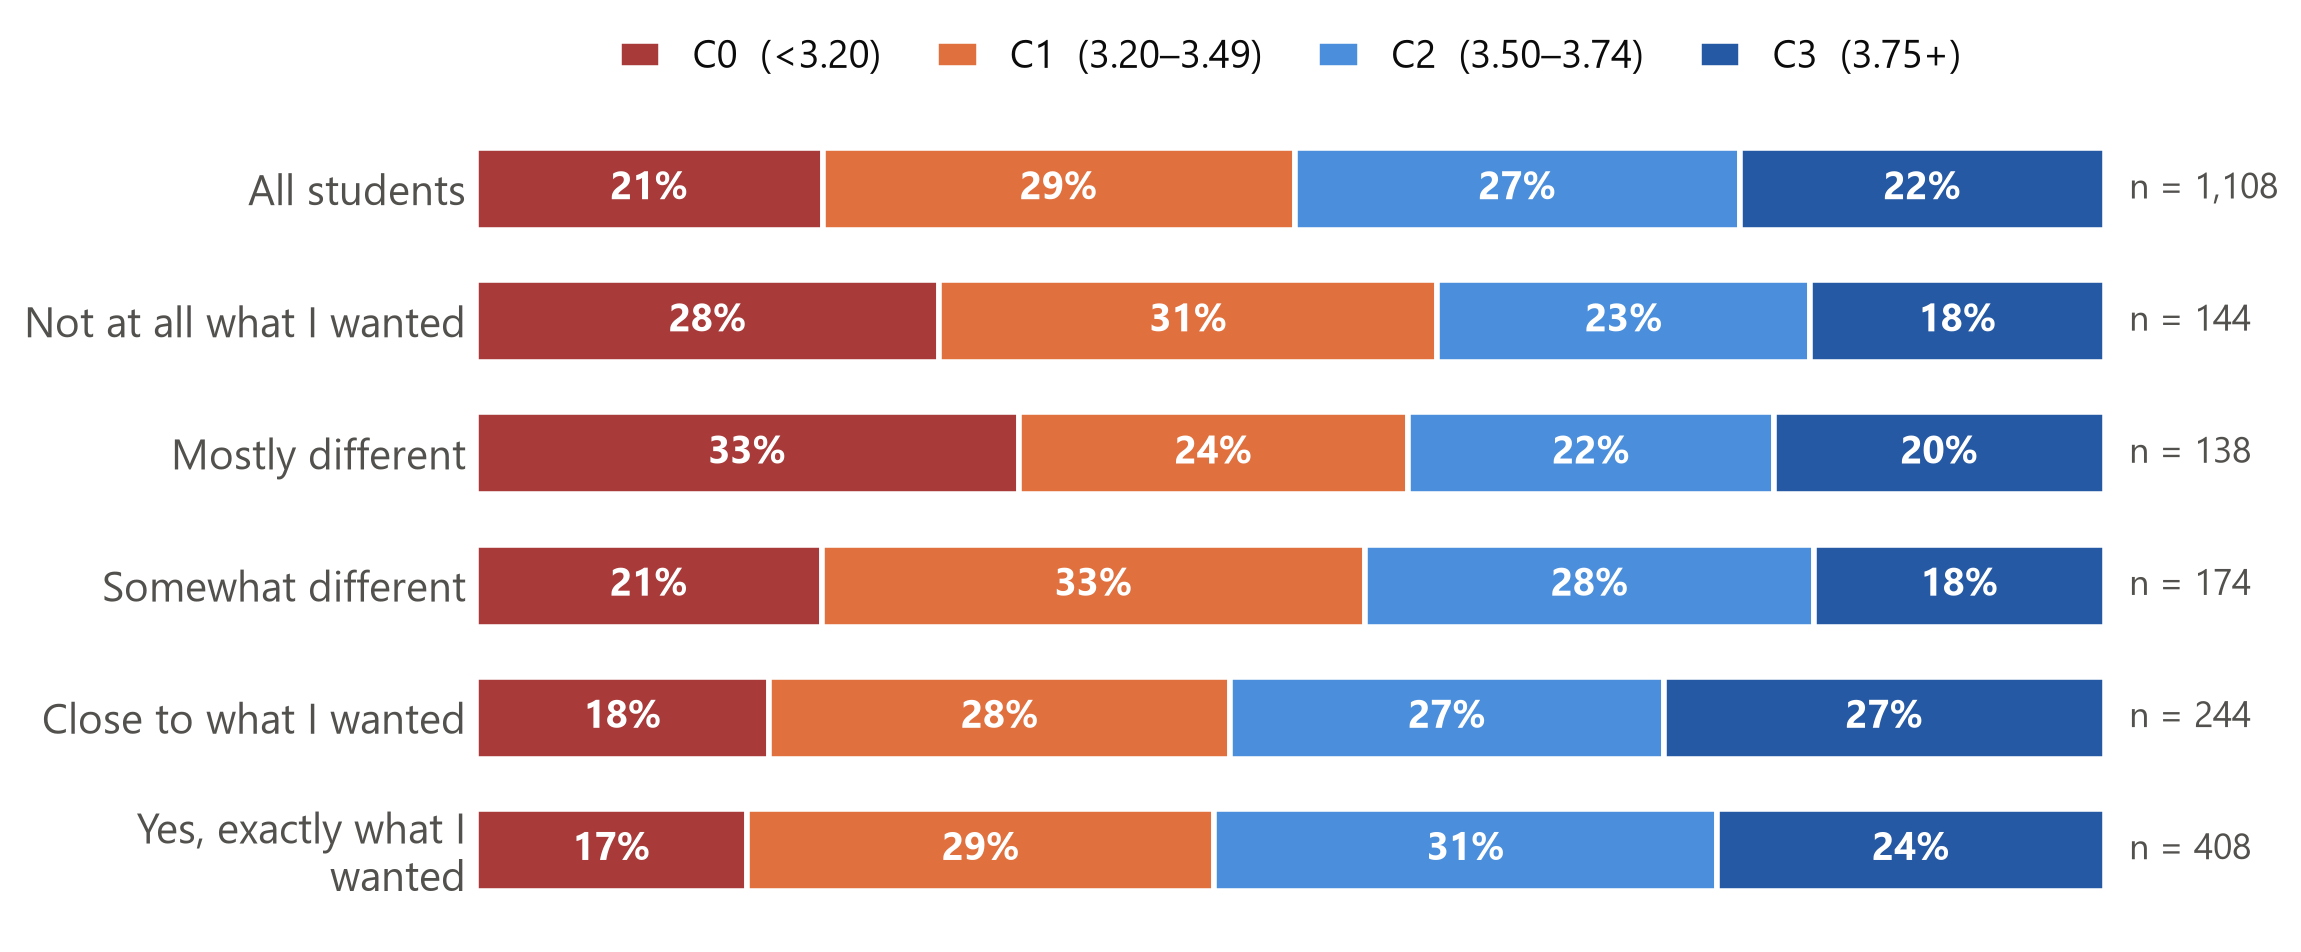
\includegraphics[width=0.9\textwidth]{figures/department_cgpa.png}
\caption{CGPA-group composition by desired-department match. The C2/C3 share is 55\% among students who report exactly the department they wanted and 41\% among those reporting no match.}
\label{fig:department-cgpa}
\end{figure}

\subsection{WEKA 10-fold cross-validation}
Table~\ref{tab:weka-cv} reports the final like-for-like model comparison on all 1,102 eligible records. J48 is the strongest SGPA model at 30.13\%, only 3.27 percentage points above ZeroR. Naive Bayes is strongest for questionnaire-only CGPA at 30.04\%, 1.00 point above ZeroR. Random Forest is strongest for the main CGPA task at 43.92\%, 14.88 points above ZeroR. These results show weak prediction from questionnaire answers alone and a clearer predictive contribution from recent SGPA.

\begin{table}[H]\centering
\caption{WEKA stratified 10-fold cross-validation accuracy on 1,102 records, seed 1.}\label{tab:weka-cv}
\begin{tabular}{lrrr}\toprule
Model&Recent SGPA (\%)&Questionnaire CGPA (\%)&Main CGPA (\%)\\\midrule
J48&30.13&26.68&38.29\\
Random Forest&29.76&29.40&\textbf{43.92}\\
SMO&25.95&27.86&37.11\\
Logistic&24.95&29.58&36.84\\
Naive Bayes&26.68&\textbf{30.04}&38.11\\
ZeroR&26.86&29.04&29.04\\\bottomrule
\end{tabular}
\end{table}

\begin{figure}[H]\centering
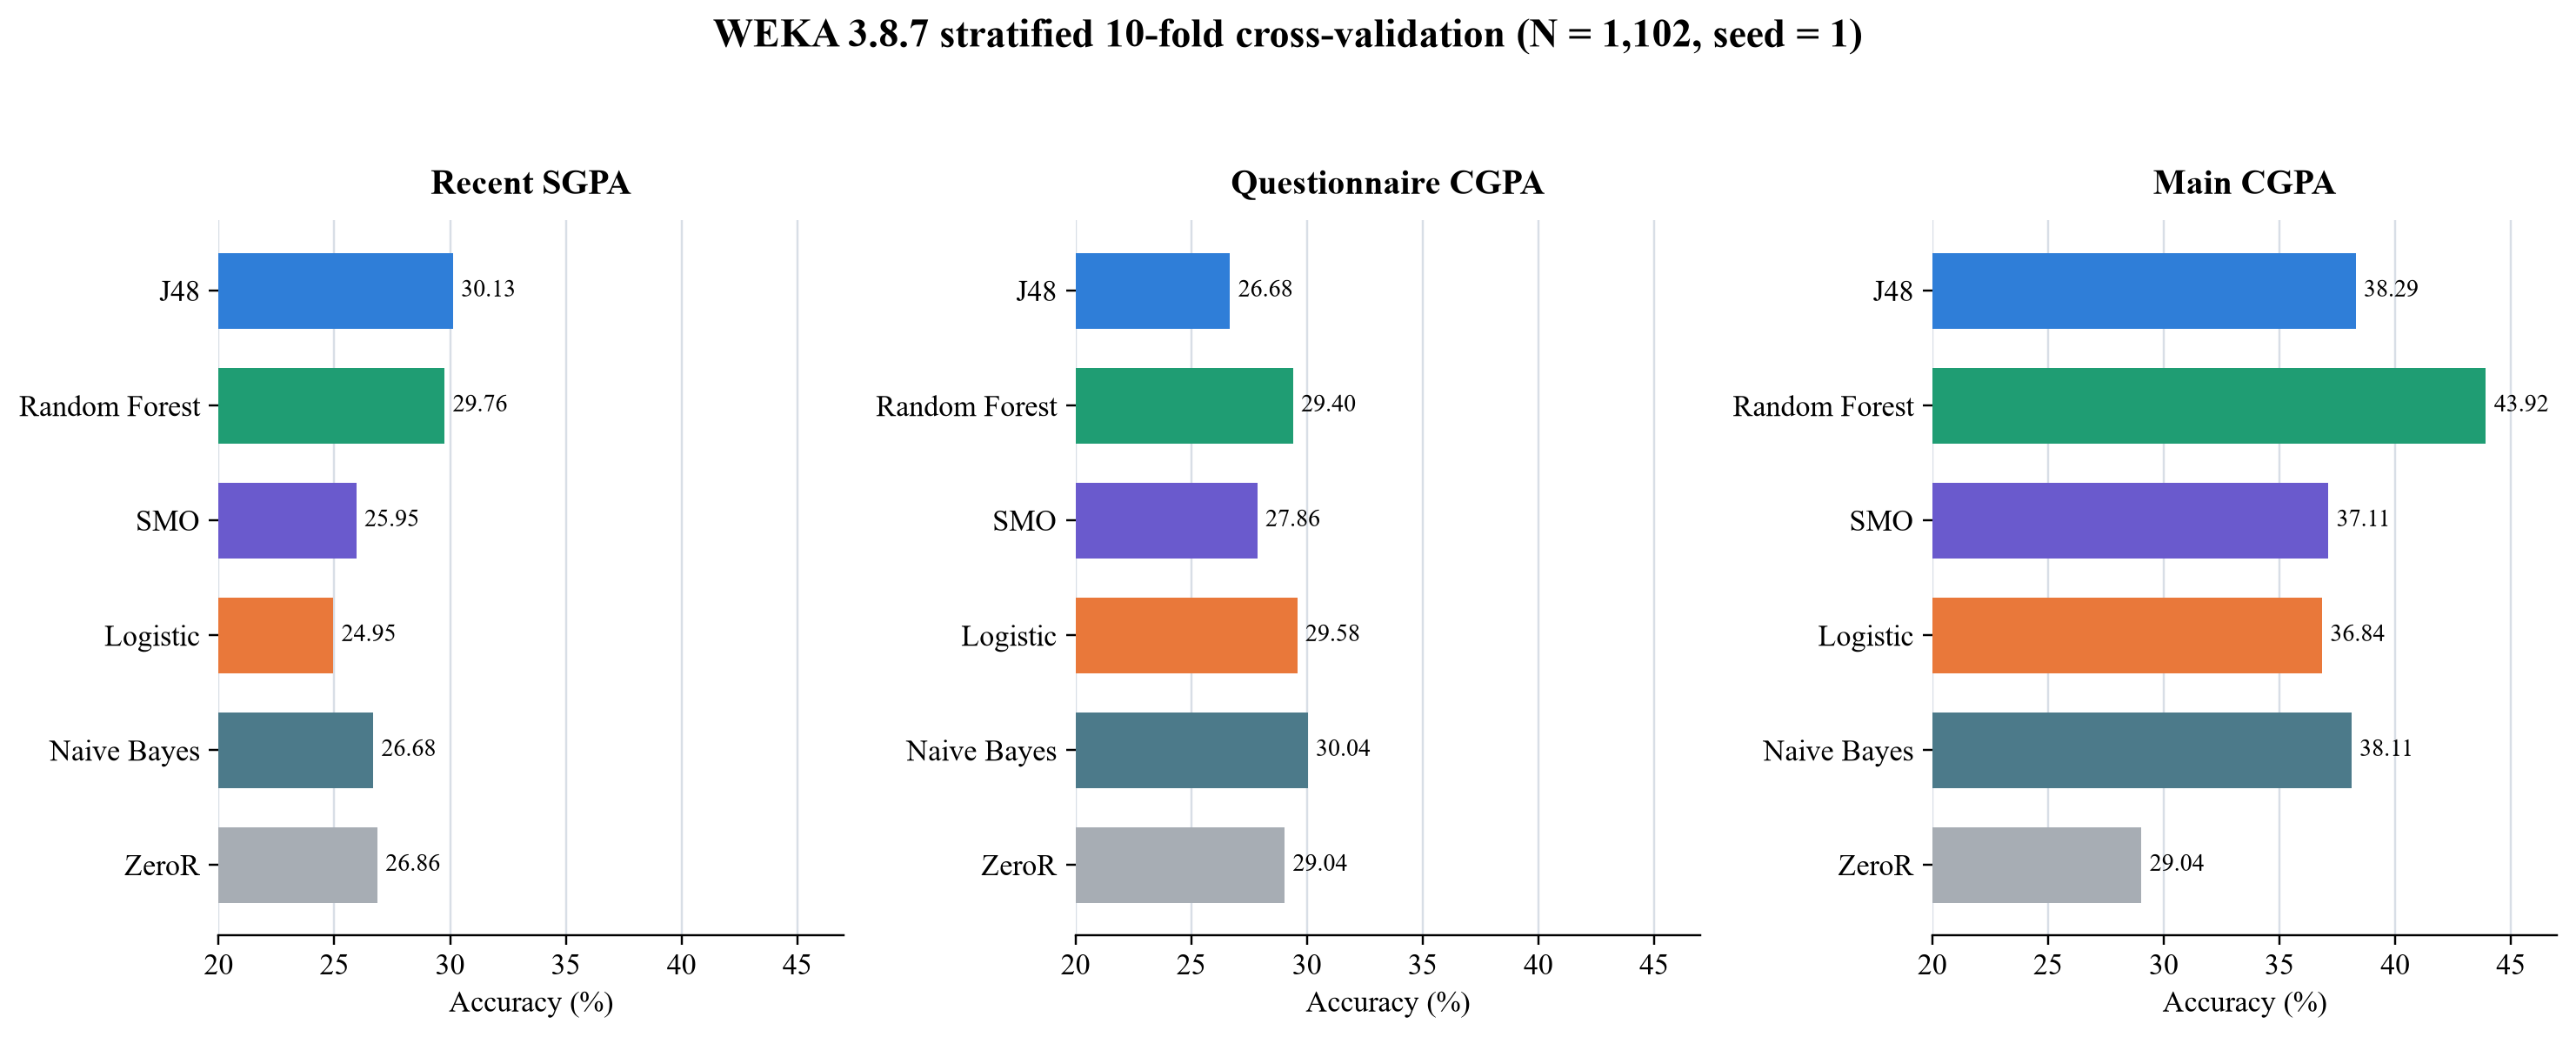
\includegraphics[width=0.96\textwidth]{figures/weka_accuracy_comparison.png}
\caption{The final WEKA cross-validation comparison. Each group uses the same 1,102 eligible students and evaluation seed.}
\label{fig:weka-accuracy}
\end{figure}

\subsection{Readable WEKA J48 trees on the fixed split}
The fixed-split J48 runs use the same 881 training and 221 test rows with \code{-C 0.25 -M 40}. The larger leaf requirement produces compact trees that can be shown without redrawing them. Table~\ref{tab:weka-holdout} reports each tree against the ZeroR test baseline.

\begin{table}[H]\centering
\caption{Fixed-split WEKA J48 results.}\label{tab:weka-holdout}
\begin{tabular}{lrrrr}\toprule
Prediction&Train (\%)&Test (\%)&Baseline (\%)&Change (pp)\\\midrule
Recent SGPA&39.39&29.86&27.15&+2.71\\
Questionnaire CGPA&36.55&32.13&28.96&+3.17\\
Main CGPA&46.20&49.77&28.96&+20.81\\\bottomrule
\end{tabular}
\end{table}

The SGPA tree begins with routine manageability and creates 13 leaves. Its 29.86\% test accuracy remains close to the 27.15\% baseline, so its branches are exploratory. Figure~\ref{fig:weka-sgpa-tree} is the actual WEKA TreeVisualizer export from this run.

\begin{figure}[H]\centering
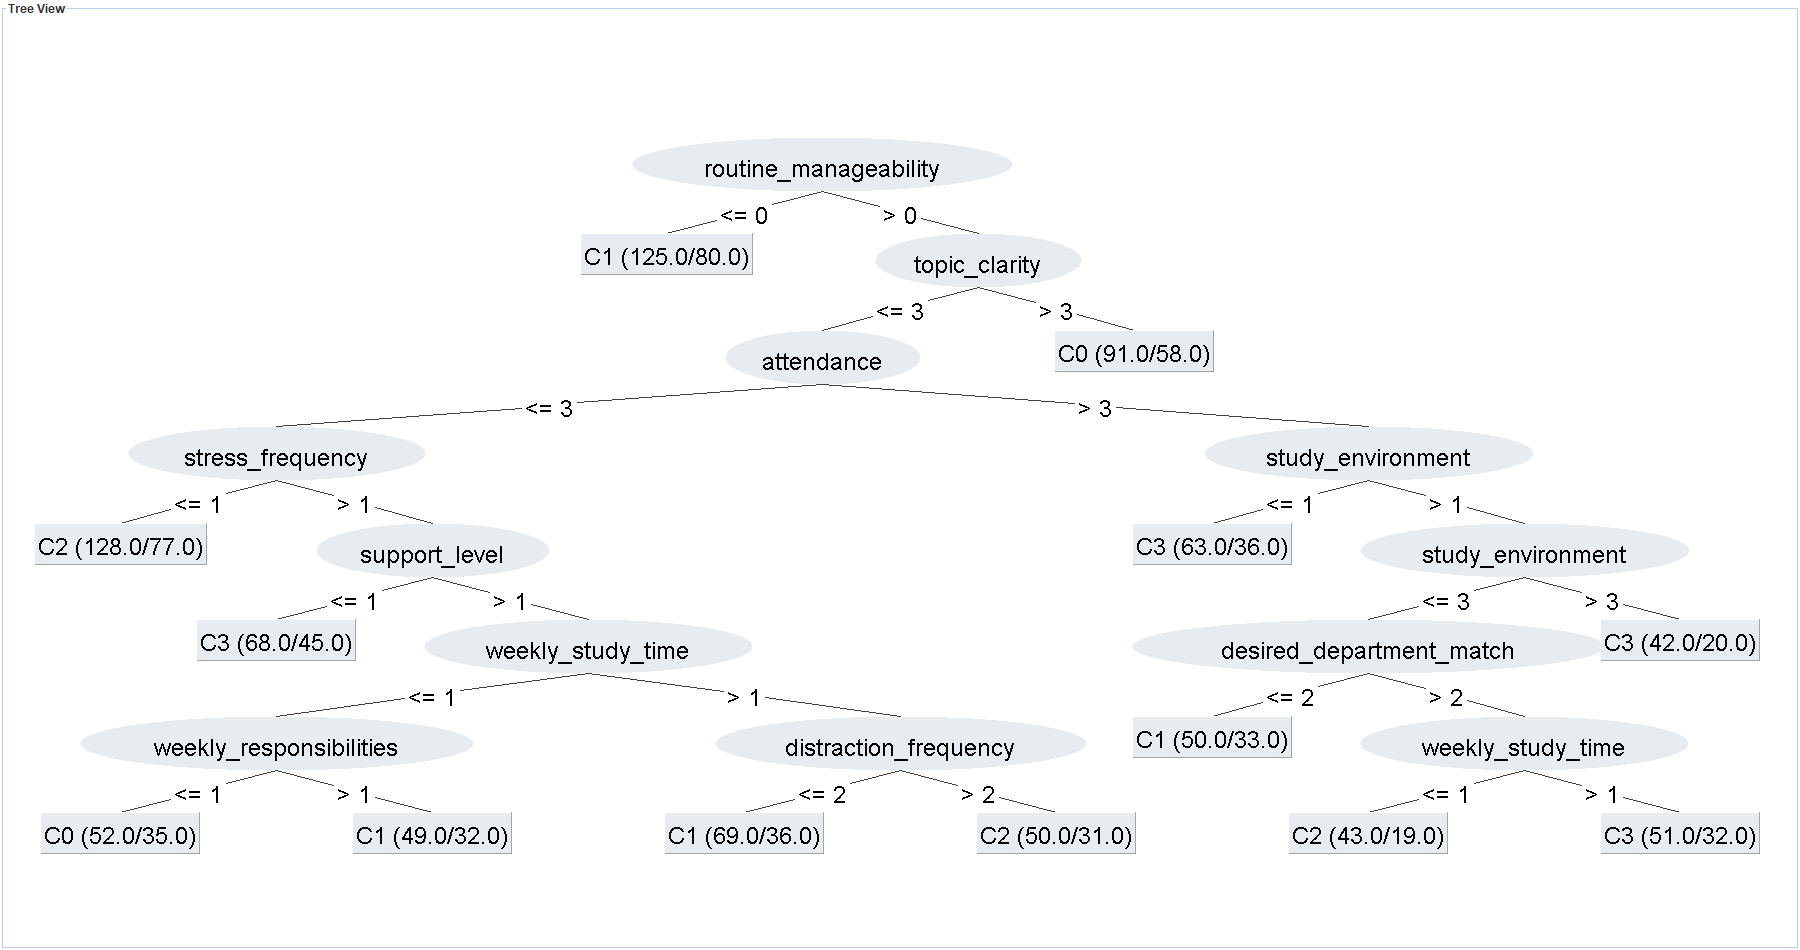
\includegraphics[width=\textwidth,height=0.70\textheight,keepaspectratio]{figures/weka_sgpa_tree.png}
\caption{Actual WEKA J48 tree for recent SGPA from the 12 questionnaire inputs.}
\label{fig:weka-sgpa-tree}
\end{figure}

The questionnaire-only CGPA tree reaches 32.13\% on the fixed test set, 3.17 points above its baseline, but the 10-fold model comparison remains near baseline. Figure~\ref{fig:weka-questionnaire-tree} shows why the result should be treated cautiously: the tree uses several survey variables while the four classes remain mixed.

\begin{figure}[H]\centering
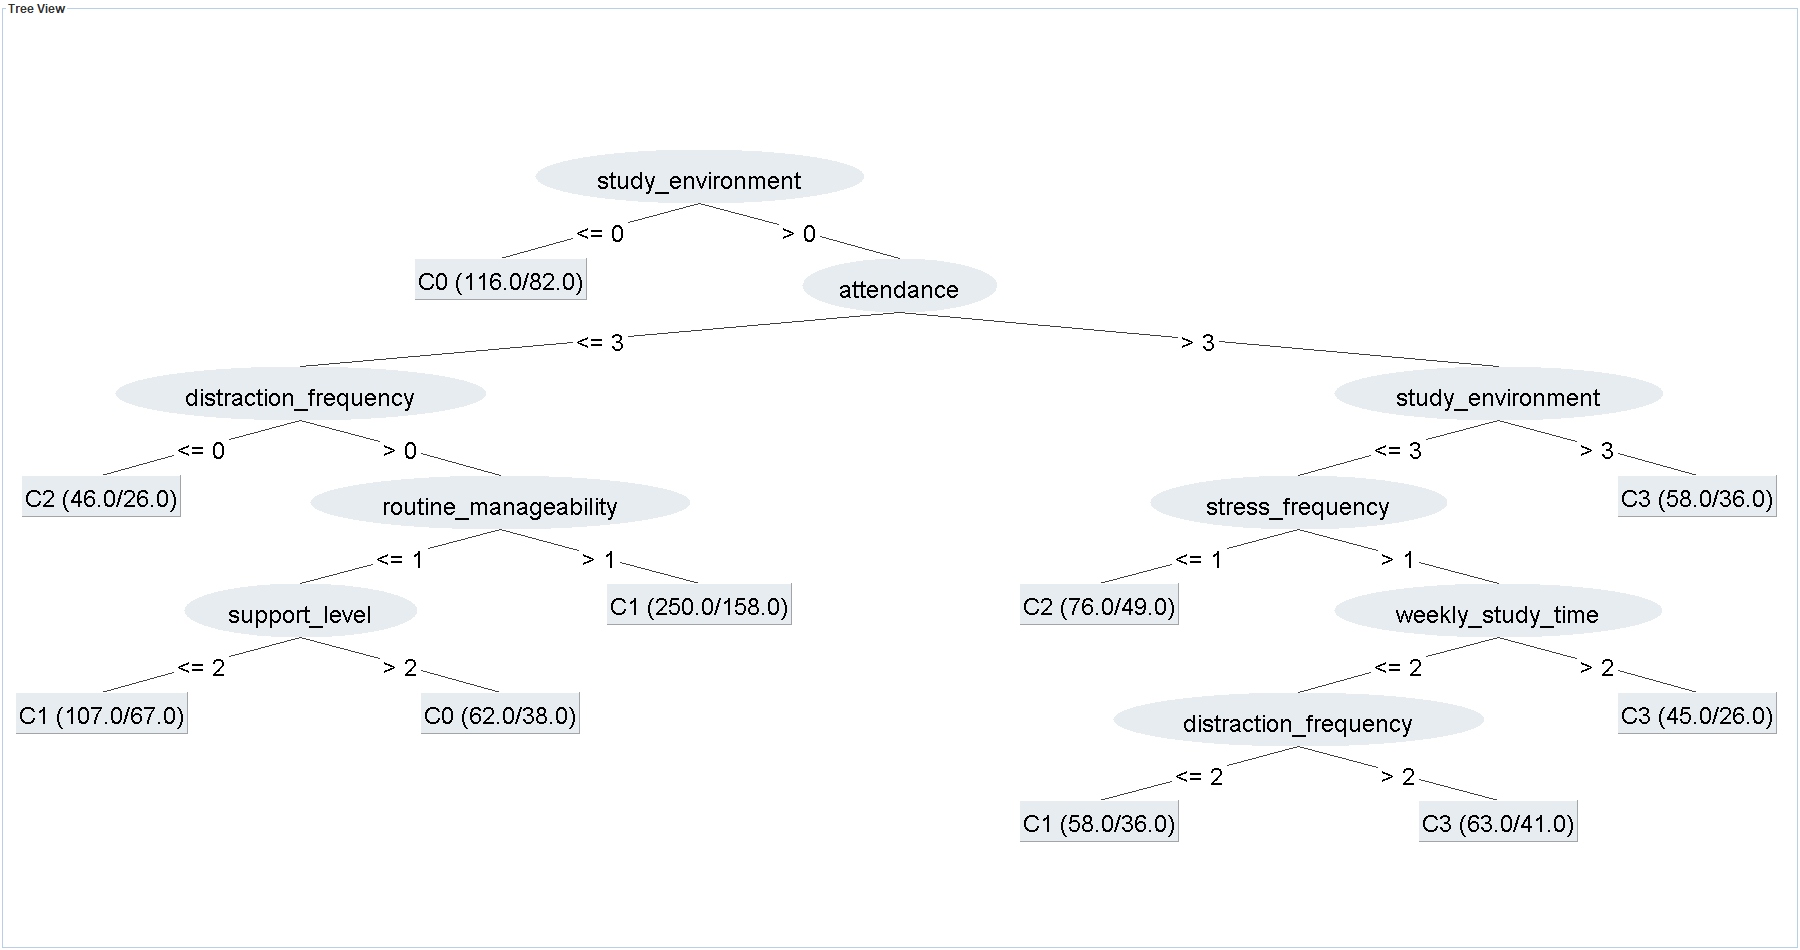
\includegraphics[width=\textwidth,height=0.70\textheight,keepaspectratio]{figures/weka_questionnaire_tree.png}
\caption{Actual WEKA J48 tree for CGPA using only the 12 questionnaire inputs.}
\label{fig:weka-questionnaire-tree}
\end{figure}

The main CGPA tree starts with recent SGPA. For students in the highest recent-SGPA band, outside commitments and desired-department match provide the remaining splits. The resulting six-leaf tree reaches 49.77\% on the fixed test set. This single-split result complements the more stable 10-fold Random Forest result; it does not replace it.

\begin{figure}[H]\centering
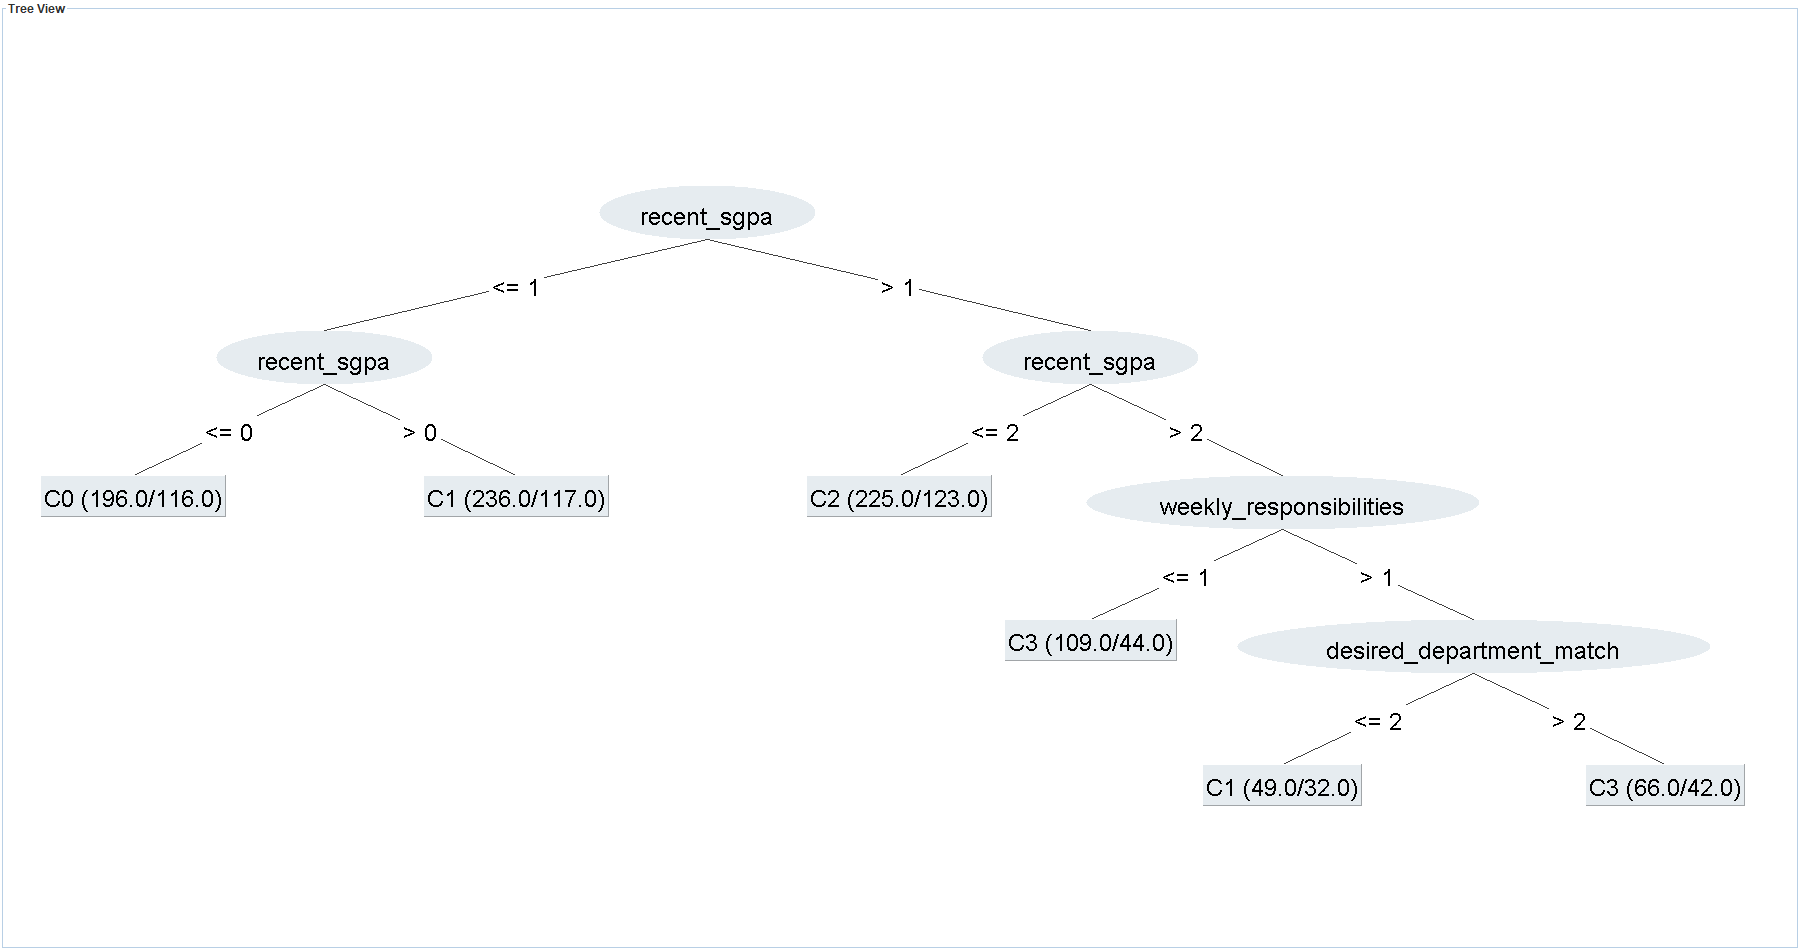
\includegraphics[width=\textwidth,height=0.65\textheight,keepaspectratio]{figures/weka_main_tree.png}
\caption{Actual WEKA J48 tree for the main CGPA task. Recent SGPA forms the first split.}
\label{fig:weka-main-tree}
\end{figure}

\subsection{Main-tree confusion matrix and ordered errors}
The main J48 tree correctly classifies 110 of 221 test students. Rows in Figure~\ref{fig:weka-main-confusion} are actual groups and columns are predicted groups. Seventy errors are one adjacent band away and 41 are two or three bands away.

\begin{figure}[H]\centering
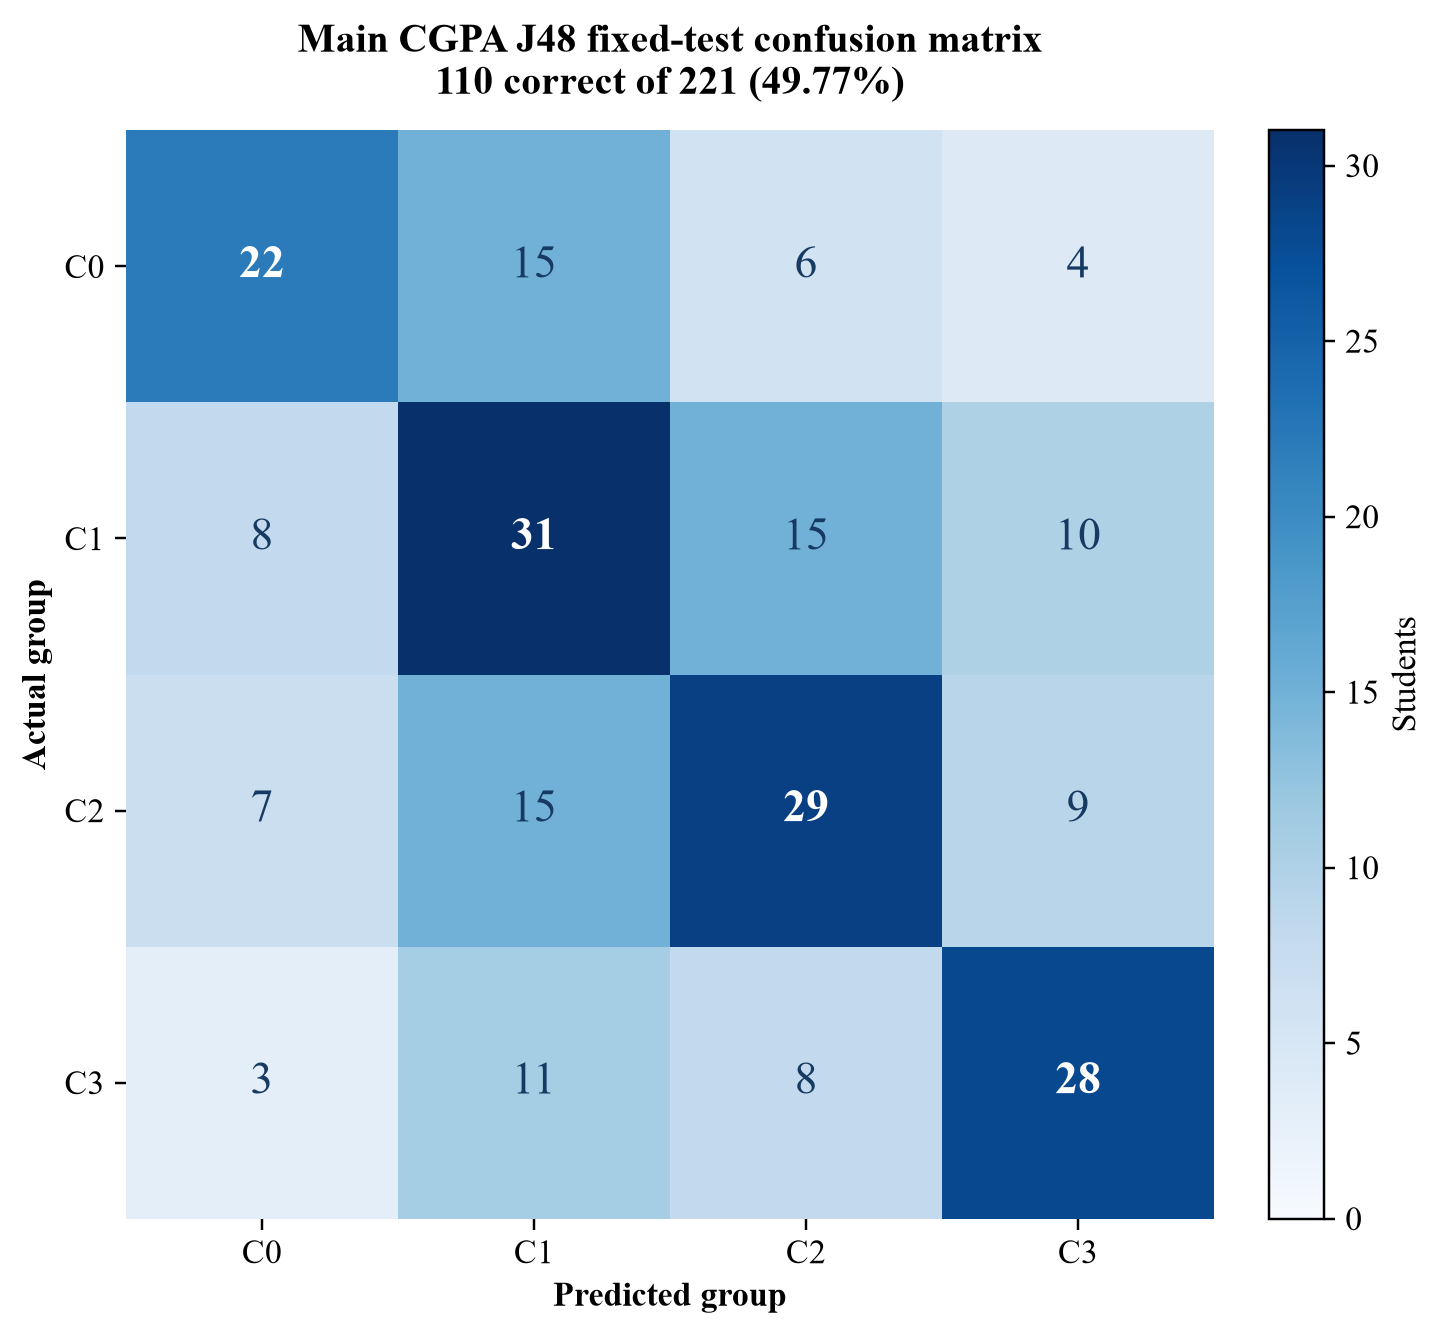
\includegraphics[width=0.78\textwidth]{figures/weka_main_confusion_matrix.png}
\caption{Fixed-test confusion matrix for the main WEKA J48 tree.}
\label{fig:weka-main-confusion}
\end{figure}

\begin{table}[H]\centering
\caption{Ordered error distribution for the 221-student fixed test set.}\label{tab:ordinal-errors}
\begin{tabular}{lrr}\toprule Absolute class distance&Students&Share (\%)\\\midrule
0: exact group&110&49.77\\
1: adjacent group&70&31.67\\
2 or 3: farther group&41&18.55\\\midrule
Mean absolute class distance&\multicolumn{2}{c}{0.719 groups}\\\bottomrule
\end{tabular}
\end{table}

\subsection{WEKA output evidence}
The repository stores the raw text log, serialized model, textual tree, DOT graph, TreeVisualizer image, and rendered output capture for each J48 target. Figure~\ref{fig:weka-output} shows the main-task output generated from the final WEKA 3.8.7 log.

\begin{figure}[H]\centering
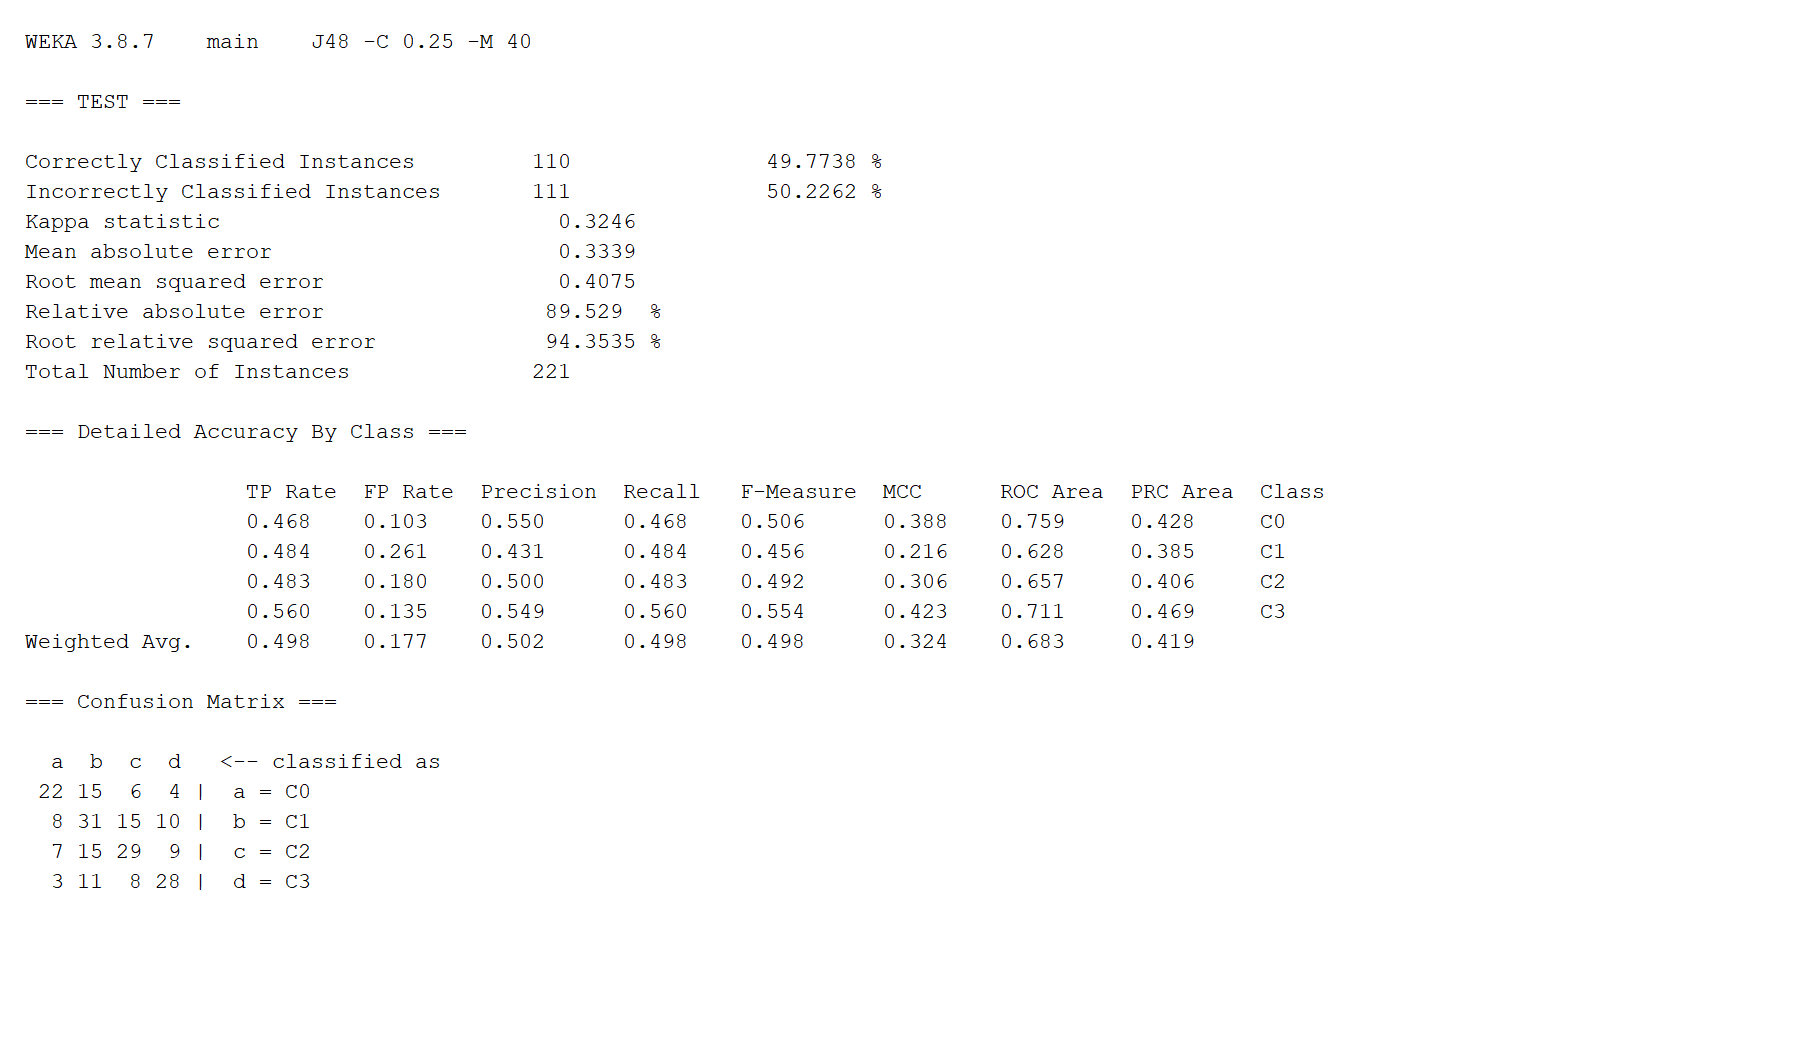
\includegraphics[width=\textwidth,height=0.72\textheight,keepaspectratio]{figures/weka_main_output.png}
\caption{Rendered WEKA output for the main CGPA J48 run, including settings, accuracy, and confusion matrix.}
\label{fig:weka-output}
\end{figure}

\subsection{Comparison with previous studies}
\begin{table}[H]\centering\scriptsize
\caption{Related-work comparison. Accuracy values use different data and targets and are not directly comparable.}\label{tab:related}
\begin{tabularx}{\textwidth}{p{0.16\textwidth}p{0.20\textwidth}p{0.23\textwidth}Y}\toprule
Study&Population or target&Models&Reported result and relation\\\midrule
Ahmed (2024) \cite{ahmed2024}&Student-performance classification&K-means, SVM, Decision Tree, Naive Bayes, KNN&SVM reported 96\% after tuning. The current work emphasises a merged engineering survey and target-specific validation.\\
Maruf et al. (2024) \cite{maruf2024}&Bangladeshi SSC and HSC results&Tuned models, stacking, SHAP&Stacking reported 82.23\% for SSC and 86.89\% for HSC. The target and population differ from four-band university CGPA.\\
Albonny and Duru (2026) \cite{albonny2026}&More than 8,000 secondary-school students; course-grade regression&Linear Regression, Decision Tree, Random Forest, DNN&Random Forest reported $R^2=93.3$. The current project uses ordinal classification and university survey data.\\
This project&1,102 eligible engineering students; CGPA C0--C3&WEKA J48, Random Forest, SMO, Logistic, Naive Bayes, ZeroR&Random Forest reaches 43.92\% under 10-fold validation; the readable J48 reaches 49.77\% on one fixed 221-row test set.\\\bottomrule
\end{tabularx}
\end{table}

\section{Discussion}
Group-level association and individual prediction answer different questions. Attendance, outside commitments, and desired-department match vary modestly across CGPA groups, but the WEKA questionnaire-only models remain close to the majority baseline. The best questionnaire-only 10-fold result is 30.04\% compared with 29.04\% for ZeroR. Students in different CGPA groups often provide similar questionnaire answers, so small distribution shifts do not create clean four-class boundaries.

Recent SGPA carries a more direct summary of academic history. When it is added to the main CGPA inputs, Random Forest reaches 43.92\% in 10-fold cross-validation. The readable J48 tree places recent SGPA at the root and uses outside commitments and desired-department match only within the highest recent-SGPA branch. That tree reaches 49.77\% on the one fixed test split. The cross-validation and fixed-split values use different model settings and should not be ranked as if they were the same experiment.

The fixed split also gives the questionnaire-only tree a small positive change from baseline, while the 10-fold comparison shows only a one-point best-model change. This variation reinforces the need to treat individual branches and single-split scores as exploratory. The stored confusion matrices, models, tree graphs, and raw WEKA logs make each reported value auditable.

The university imbalance limits how far the findings can generalise. The one-time self-reported design prevents causal conclusions. Questionnaire imputation was fitted before evaluation in the historical cleaning pipeline, so limited preprocessing leakage may make the scores optimistic. The results support language such as ``associated with,'' ``more common among,'' and ``helps prediction.'' They do not support claims that a questionnaire answer causes a grade or guarantees a student's outcome.

Future data collection should prioritise verified grades, course-level results, repeated observations of the same students, objective activity indicators, and better-balanced university sampling. A future evaluation should fit every imputation step inside each training fold before using the system for any decision beyond classroom demonstration.

\section{Conclusion}
\textbf{Dataset.} Two related Google Forms were harmonised into a documented dataset of 1,108 engineering students from four universities. The workflow preserves raw files, mappings, cleaned tables, figures, ARFF datasets, and audit logs.

\textbf{Data understanding.} The survey responses vary across all answer options. Desired-department match, attendance, and outside commitments show the clearest corrected CGPA associations, but the effect sizes remain small.

\textbf{WEKA analysis.} Every final model experiment uses the same 1,102 eligible records. Questionnaire-only prediction is weak: the best 10-fold result reaches 30.04\% against a 29.04\% CGPA baseline. For the main CGPA task, Random Forest reaches 43.92\% in 10-fold validation. The readable fixed-split J48 tree reaches 49.77\% on 221 test students and relies first on recent SGPA. The exact WEKA trees, models, logs, and confusion matrices are included with the project.

The findings describe associations and predictive patterns in the collected survey data. They do not establish causal effects, and the stated sampling and preprocessing limitations remain part of every result.

\section{Ethics, authorship, and declarations}
\subsection{Ethics and privacy}
The working dataset omits direct identifiers from modelling, and the presentation assets avoid exposing individual responses. The analysis reports aggregated counts, distributions, and model results. It must not be used for grading, discipline, scholarships, or other decisions about individual students.

\placeholder{Insert the exact statement that reflects the course survey's actual consent and institutional ethics procedure. Do not add an approval number or consent claim unless the team can verify it.}

\subsection{CRediT author statement}
\placeholder{Confirm each team member's actual roles before submission, then list only verified contributions such as conceptualisation, data collection, methodology, software, validation, visualisation, writing, and presentation.}

\subsection{Acknowledgements and funding}
\placeholder{Add verified acknowledgements and the accurate funding statement. If the work received no external funding, confirm that fact before inserting the standard no-funding declaration.}

\subsection{Competing interests}
\placeholder{Insert the team's confirmed competing-interests declaration.}



\printbibliography[title={References}]
\appendix
\section{Questionnaire and data dictionary summary}
The complete, bilingual questionnaire and detailed coding dictionary remain in the project package. Table~\ref{tab:dictionary} provides the modelling variables used in the teacher-facing experiments.
\begin{longtable}{p{0.24\linewidth}p{0.23\linewidth}p{0.16\linewidth}p{0.27\linewidth}}
\caption{Teacher-facing modelling data dictionary.}\label{tab:dictionary}\\
\toprule Feature & Meaning & Type & Missing-value treatment\\\midrule\endfirsthead
\toprule Feature & Meaning & Type & Missing-value treatment\\\midrule\endhead
attendance & Class attendance band & Ordinal & Modal response within source when blank\\
weekly\_study\_time & Self-study hours per week & Ordinal & Modal response within source when blank\\
study\_style & Regularity of study & Ordinal & Harmonised label, then within-source fill\\
topic\_clarity & Topic clarity after class & Ordinal & Within-source fill\\
sleep\_duration & Sleep on a normal night & Ordinal & Within-source fill\\
stress\_frequency & Stress blocking study & Ordinal & Within-source fill\\
weekly\_responsibilities & Tuition, job, club hours & Ordinal & Blank mapped to None when supported by form evidence\\
distraction\_frequency & Digital distraction & Ordinal & Within-source fill\\
study\_environment & Suitability of living place & Ordinal & Within-source fill\\
support\_level & Family or friend support & Ordinal & Within-source fill\\
desired\_department\_match & Match with preferred department & Ordinal & Within-source fill\\
routine\_manageability & Semester routine management & Ordinal & Within-source fill\\
recent\_sgpa & Most recent SGPA group & Ordinal band & Six affected rows excluded from tree experiments\\
cgpa & Cumulative CGPA group & Ordered target & Records without usable target removed\\
\bottomrule
\end{longtable}

\section{Full model result tables}
\begin{table}[H]\centering\small
\caption{Final WEKA 10-fold cross-validation accuracy on 1,102 eligible students, seed 1.}\label{tab:weka-full}
\begin{tabular}{lrrr}\toprule
Model&Recent SGPA&Questionnaire CGPA&Main CGPA\\\midrule
J48&30.13&26.68&38.29\\
Random Forest&29.76&29.40&43.92\\
SMO&25.95&27.86&37.11\\
Logistic&24.95&29.58&36.84\\
Naive Bayes&26.68&30.04&38.11\\
ZeroR&26.86&29.04&29.04\\\bottomrule
\end{tabular}
\end{table}

\section{Reproducibility checklist}
\begin{itemize}
\item Current merged pipeline: \path{notebooks/02_merged_cleaning_eda_modeling.ipynb} and \path{notebooks/pipeline_v2_source.py}.
\item Teacher-facing analysis: \code{notebooks/03\_teacher\_focused\_analysis.ipynb}.
\item Descriptive snapshot: 1,108 records. All model experiments: 1,102 records after excluding six target-conditioned SGPA imputations.
\item Final WEKA evidence: nine ARFF files, 18 cross-validation logs, three fixed-split J48 logs, serialized models, exact trees, and audit files under \path{weka-final/evidence/}.
\item Model comparison: stratified 10-fold cross-validation with seed 1. Explanatory J48: the existing CGPA-stratified 881/221 split with seed 42, reused for all targets.
\item Cross-validation J48 uses \code{-C 0.25 -M 2}; explanatory J48 uses \code{-C 0.25 -M 40}.
\item Run the scripts in \path{weka-final/scripts/} to rebuild and audit the final evidence package.
\end{itemize}

\end{document}
